\chapter{Experimental Results}\label{ch:m-results}

This chapter presents the results in the order the experiments were run (Section~\ref{sec:research-planning-levels}): first the communication microbenchmarks, then the \texttt{moe} and \texttt{cg\_step} application microbenchmarks, and finally the aCG solver. Across all of them, the performance of a backend depends strongly on the communication pattern and on the configuration of the underlying libraries.

Each section follows the same topology progression, from \texttt{1n2g} and \texttt{1n4g} on NVLink, through \texttt{2n1g} on a single InfiniBand link, to \texttt{2n4g}--\texttt{8n4g} with both domains active. The question it answers throughout is whether a stack that performs well within a node keeps that advantage once communication crosses the network.

Benchmark curves show the median of allocation means with their range, as defined in Section~\ref{sec:execution-procedure}; the main figures use representative topologies, and the complete panels are in Appendix~\ref{app:complete-results}. Results available only as summaries are identified where they appear, and the preliminary NCCL study is kept in Appendix~\ref{app:nccl-preliminary}.

\section{Communication Microbenchmarks}\label{sec:micro-results}

Each pattern shows all backends measured in its campaign. The accompanying explanation identifies the runtime settings, batching, and completion behavior that affect the comparison.

\subsection{Ping-Pong}

The first comparison asks whether device-side invocation improves a dependency-ordered exchange. Figure~\ref{fig:m-pingpong-regimes} shows all six measured paths. Across nodes, CUDA MPI has the lowest latency throughout the sweep. At four bytes its allocation-based median is 3.36\,$\mu$s, compared with 7.28\,$\mu$s for OSHMPI, 17.17\,$\mu$s for NVSHMEM, and 28.78\,$\mu$s for NCCL. Device invocation therefore does not remove the startup advantage of the evaluated MPI path.

\begin{figure}[htbp]
\centering
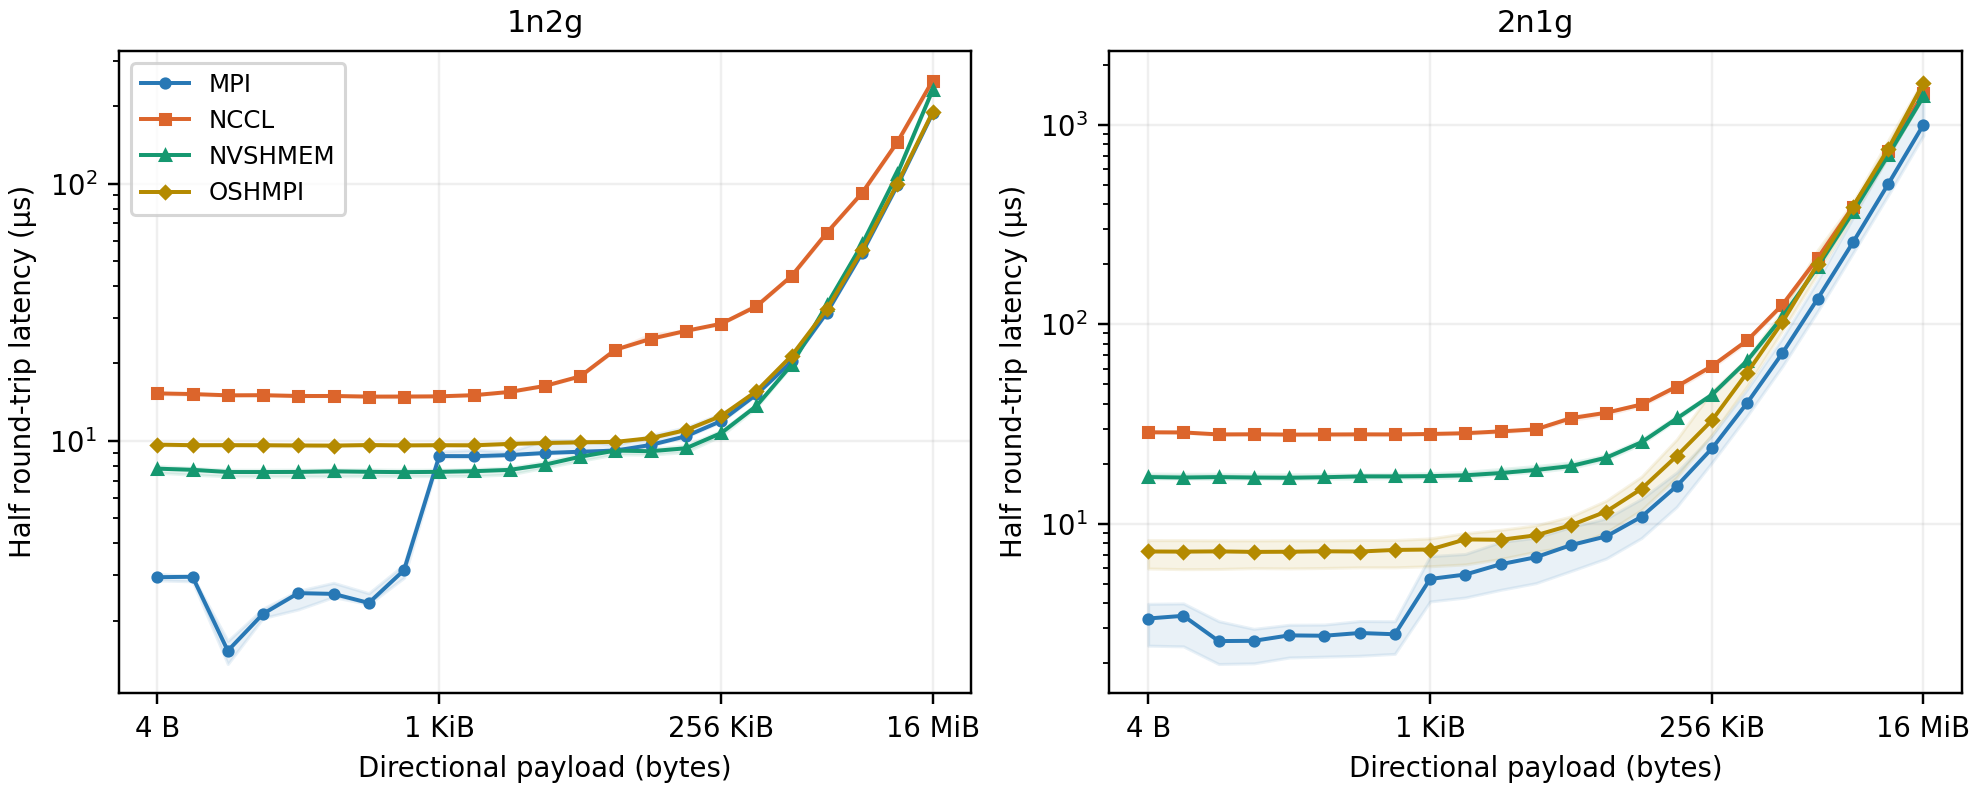
\includegraphics[width=\textwidth]{figures/results/pingpong-regimes.png}
\caption[\texttt{pingpong} latency within one node and across two nodes]{\texttt{pingpong} latency for all six measured stacks within one node and across two nodes. Points are medians of five allocation means; shading spans those means. Latency is half the round-trip time.}
\label{fig:m-pingpong-regimes}
\end{figure}

Within a node, NVSHMEM becomes competitive over an intermediate message range, while MPI again improves relative to it at large payloads. Table~\ref{tab:m-pingpong-inter} also shows that CUDA and SYCL MPI are close for small messages but differ substantially at the largest payloads. Sharing an MPI installation therefore does not guarantee identical execution costs at every size.

\begin{table}[htbp]
\centering
\caption[Inter-node \texttt{pingpong} latency on \texttt{2n1g}]{Inter-node \texttt{pingpong} latency on \texttt{2n1g}, including SYCL paths. Values are allocation-based medians in \,$\mu$s.}
\label{tab:m-pingpong-inter}
\footnotesize
% Generated by tools/rebuild_main_evidence.py; include outside tabular.
\begin{tabular}{lrr}
\toprule
Stack & 4\,B & 16\,MiB\\
\midrule
MPI & 3.358 & 1000.370\\
SYCL MPI & 3.094 & 1736.543\\
OSHMPI & 7.275 & 1614.043\\
NVSHMEM & 17.171 & 1388.240\\
NCCL & 28.781 & 1436.673\\
oneCCL/NCCL & 33.789 & 1444.770\\
\bottomrule
\end{tabular}

\end{table}

Small-message ping-pong also makes the overhead of oneCCL/NCCL visible. At four bytes across nodes, it takes 33.8\,$\mu$s against 28.8\,$\mu$s for direct NCCL, approximately 17\% more. This comparison changes the compute interface and host coordination as well as the adapter call, so the difference includes all three. The timings describe half a round trip; they do not isolate either adapter overhead or kernel-launch savings.

\begin{keypoint}[Ping-pong takeaway]
MPI has the lowest latency at every size across nodes and provides the startup-cost reference. OSHMPI is the closest alternative for small messages, at roughly twice MPI's four-byte latency. NVSHMEM is competitive over an intermediate intra-node range, but GPU initiation does not remove its small-message disadvantage. NCCL is an order of magnitude slower at four bytes in a timing that includes waiting for its stream to finish. oneCCL/NCCL adds about 17\% to direct NCCL, and SYCL MPI tracks CUDA MPI at small sizes but not at the largest ones.
\end{keypoint}

\subsection{Halo Exchange}

A repeated neighbor exchange offers a different opportunity from ping-pong. The fixed submission and completion cost can be spread across many exchanges, while multiple peer transfers can proceed together. Figure~\ref{fig:m-halo-regimes} contrasts isolated and steady-state execution on one and eight nodes.

\begin{figure}[htbp]
\centering
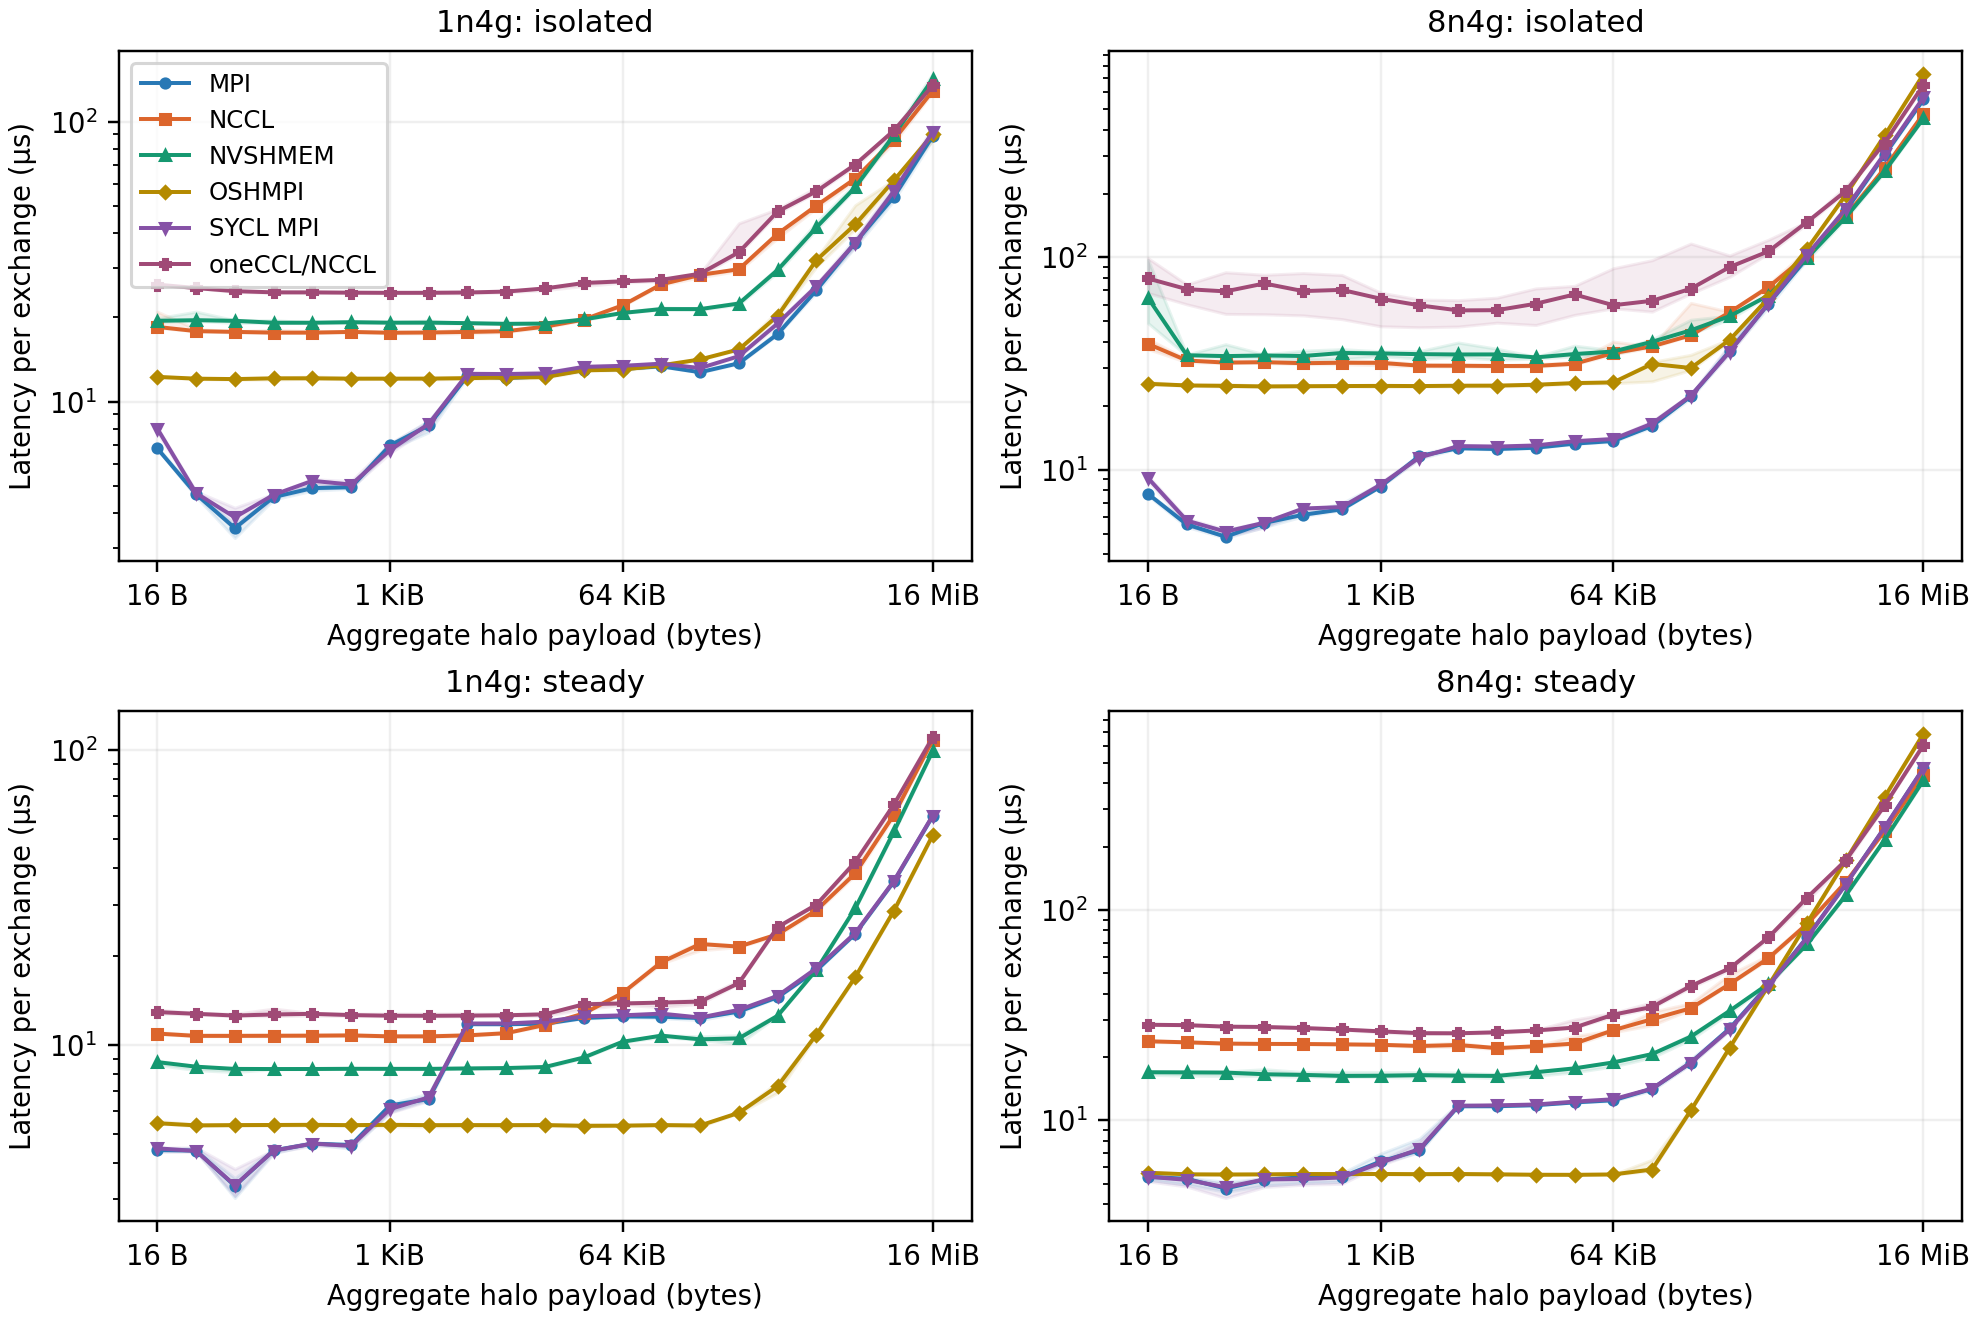
\includegraphics[width=\textwidth]{figures/results/halo-regimes.png}
\caption[Isolated and steady-state halo latency]{Isolated and steady-state halo latency for all six measured stacks. Steady-state values amortize a batch of 100 exchanges. Points and shading show allocation medians and ranges; payload counts two sends and two receives.}
\label{fig:m-halo-regimes}
\end{figure}

MPI supplies the low-startup reference for isolated exchanges. Batching makes OSHMPI competitive across small and intermediate payloads because its batch-level completion cost is amortized. At large multi-node payloads, persistent NVSHMEM sustains the highest rate among the direct paths in Table~\ref{tab:m-halo-bandwidth}. Its approximately 41\,GB/s aggregate rate remains similar from two to eight nodes, while MPI reaches approximately 34--36\,GB/s.

\begin{table}[htbp]
\centering
\caption[Peak steady-state halo bandwidth]{Peak steady-state halo bandwidth computed from allocation-median latency, in GB/s. The numerator is aggregate logical halo volume, not one NIC's traffic.}
\label{tab:m-halo-bandwidth}
% Generated by tools/rebuild_main_evidence.py; include outside tabular.
\begin{tabular}{lrrr}
\toprule
Topology & CUDA MPI & CUDA NVSHMEM & OSHMPI\\
\midrule
\texttt{2n4g} & 34.4 & 41.1 & 24.5\\
\texttt{4n4g} & 36.5 & 40.9 & 24.4\\
\texttt{8n4g} & 35.7 & 40.6 & 24.4\\
\bottomrule
\end{tabular}

\end{table}

Persistent NVSHMEM performs best when neighbor exchanges are repeated long enough to spread the fixed costs over a batch. SYCL MPI and oneCCL/NCCL show the same distinction between isolated and sustained exchanges. The host-driven OSHMPI result is important for RQ1: batching and the choice of when to wait can help even when the GPU does not initiate communication. Since signaling, persistence, sampling, and progress differ between implementations, the measurements cannot assign the NVSHMEM advantage solely to fewer launches. Its inter-node measurements use the CPU proxy described in Section~\ref{sec:ibgda-check}.

\begin{keypoint}[Halo takeaway]
The fastest stack depends on whether exchanges are measured individually or in batches. MPI is the reference for isolated exchanges, where each measurement includes submission and completion. OSHMPI becomes competitive when a batch spreads its completion cost across many exchanges, but reaches only about 24.4\,GB/s across multi-node topologies, the lowest sustained rate measured. Persistent GPU-initiated NVSHMEM sustains the highest multi-node rate, 40.6--41.1\,GB/s, against 34.4--36.5\,GB/s for MPI. NCCL and oneCCL/NCCL show the same isolated-versus-batched distinction, and SYCL MPI again tracks CUDA MPI.
\end{keypoint}

\subsection{Allreduce}

For reductions, small scalar sums emphasize startup latency while large buffers emphasize throughput. Figure~\ref{fig:m-allreduce-backends} shows all seven measured stacks at representative intra- and multi-node topologies. NCCL-based implementations lead for large messages (Table~\ref{tab:m-allreduce-bandwidth}). Within a node, NVSHMEM matches NCCL closely (128.3 against 127.5\,GB/s on \texttt{1n4g}) because the benchmark enables NVSHMEM's dispatch of collectives to NCCL. This agreement measures delegated NCCL execution, not NVSHMEM's own reduction algorithm.

The two series diverge across nodes. At \texttt{4n4g}, NVSHMEM reaches 14.3\,GB/s against NCCL's 31.8\,GB/s; at \texttt{8n4g}, the figures are 11.9 and 29.5\,GB/s. For the 16\,MiB reduction, NVSHMEM takes 2733\,$\mu$s against NCCL's 1104\,$\mu$s. Its timings also vary more widely between allocations.

The selected collective implementation may explain part of this difference. NVSHMEM delegates to NCCL within a node, but the archive lacks the per-run dispatch information needed to confirm what ran across nodes. The timings describe the measured stack, but do not support a ranking of the underlying collective algorithms.

\begin{figure}[htbp]
\centering
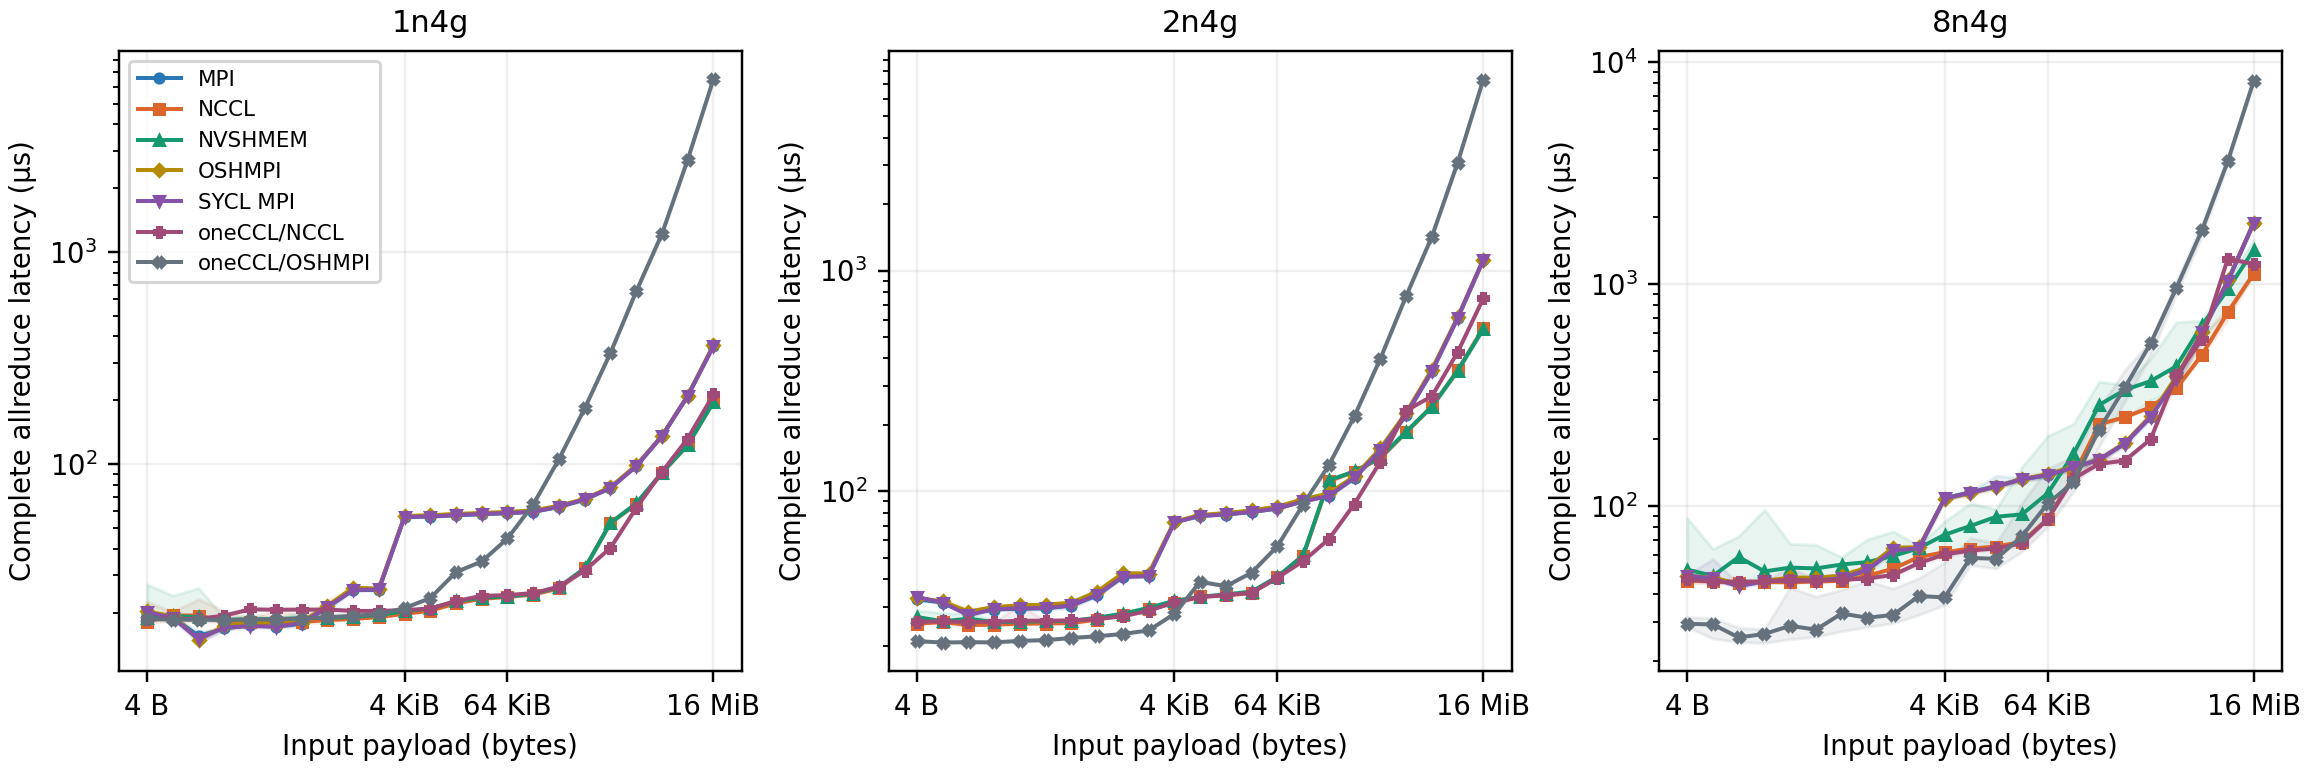
\includegraphics[width=\textwidth]{figures/results/allreduce-backends.png}
\caption[\texttt{allreduce} latency at representative topologies]{\texttt{allreduce} latency for all seven measured stacks at representative topologies. Points are medians of allocation means and shading spans those means. The input payload is per rank; the single-rank control is discussed separately.}
\label{fig:m-allreduce-backends}
\end{figure}

\begin{table}[htbp]
\centering
\caption[Peak \texttt{allreduce} bus bandwidth]{Peak \texttt{allreduce} bus bandwidth in GB/s, recomputed as input bytes divided by allocation-median latency and multiplied by $2(P-1)/P$.}
\label{tab:m-allreduce-bandwidth}
% Generated by tools/rebuild_main_evidence.py; include outside tabular.
\begin{tabular}{lrrr}
\toprule
Topology & CUDA NCCL & CUDA NVSHMEM & CUDA MPI\\
\midrule
\texttt{1n4g} & 127.7 & 128.3 & 69.7\\
\texttt{2n4g} & 53.5 & 54.0 & 26.3\\
\texttt{4n4g} & 32.1 & 31.7 & 20.0\\
\texttt{8n4g} & 29.2 & 22.9 & 17.3\\
\bottomrule
\end{tabular}

\end{table}

The OSHMPI comparison shows how staging can change the cost of a common interface. On \texttt{1n4g}, the four-byte allreduce medians are 20.2\,$\mu$s directly and 18.6\,$\mu$s through oneCCL/OSHMPI. At 16\,MiB, they are 364\,$\mu$s and 6538\,$\mu$s, respectively: the adapter is approximately 18 times slower. Direct OSHMPI reduces device-resident operands, whereas the adapter stages them through symmetric buffers and uses different completion steps. The gap measures this integration choice; other oneCCL backends need not incur the same cost.

This pattern demonstrates why functional interface compatibility and performance retention must be evaluated separately. The OSHMPI adapter waits for queue dependencies, stages ordinary operands through symmetric storage, performs a blocking host operation, and returns an already-complete event. Those semantics preserve correctness but remove the asynchronous opportunity retained by the NCCL path.

\begin{keypoint}[Allreduce takeaway]
Payload size changes the ranking. MPI and OSHMPI are fastest at four bytes across nodes, at 12.4 and 12.6\,$\mu$s on \texttt{2n1g} against about 20\,$\mu$s for the others. NVSHMEM matches NCCL within a node through dispatch, but its multi-node results diverge and need the configuration qualification above. NCCL leads at 16\,MiB, taking 1104\,$\mu$s at \texttt{8n4g} against 1879\,$\mu$s for MPI. oneCCL/NCCL follows it closely, while oneCCL/OSHMPI is about 18 times slower than direct OSHMPI for the 16\,MiB intra-node reduction. SYCL MPI remains close to CUDA MPI. Runtime tuning is also decisive: UCC changes MPI's 16\,MiB result by up to 96.5 times.
\end{keypoint}

\subsubsection{UCC Impact}

The UCC control explains why MPI's result cannot be summarized by a single library label, and it is the largest configuration effect measured anywhere in this campaign. Figure~\ref{fig:m-ucc-allreduce} shows both configurations in absolute terms, because the ratio alone understates what is at stake. At a 16\,MiB intra-node reduction on \texttt{1n4g}, the same MPI installation takes 34.9\,ms with UCC disabled and 361\,$\mu$s with it enabled, a factor of 96.5. The corresponding multi-node figures are 39.6\,ms against 1121\,$\mu$s at \texttt{2n4g} and 45.2\,ms against 1873\,$\mu$s at \texttt{8n4g}. The non-UCC curve does not merely scale worse: it breaks down above 1\,MiB, where doubling the payload to 2\,MiB multiplies its cost by 5.1, from 809\,$\mu$s to 4101\,$\mu$s, and the gap widens monotonically from there.

The trade-off runs the other way at small payloads, which is why the policy is a choice rather than a default to enable everywhere. Around 4\,KiB, UCC is slower on every measured topology, by factors of 0.55, 0.54, and 0.46 at \texttt{1n4g}, \texttt{2n4g}, and \texttt{8n4g}. Intra-node the curve recovers quickly; on the two multi-node topologies UCC remains behind until roughly 64\,KiB. The reductions that \texttt{cg\_step} and aCG actually perform are single doubles, which sit firmly inside that penalty region, and this is why Section~\ref{sec:runtime-method} disables UCC for the \texttt{cg\_step} benchmark while enabling it for the standalone sweep.

\begin{figure}[htbp]
\centering
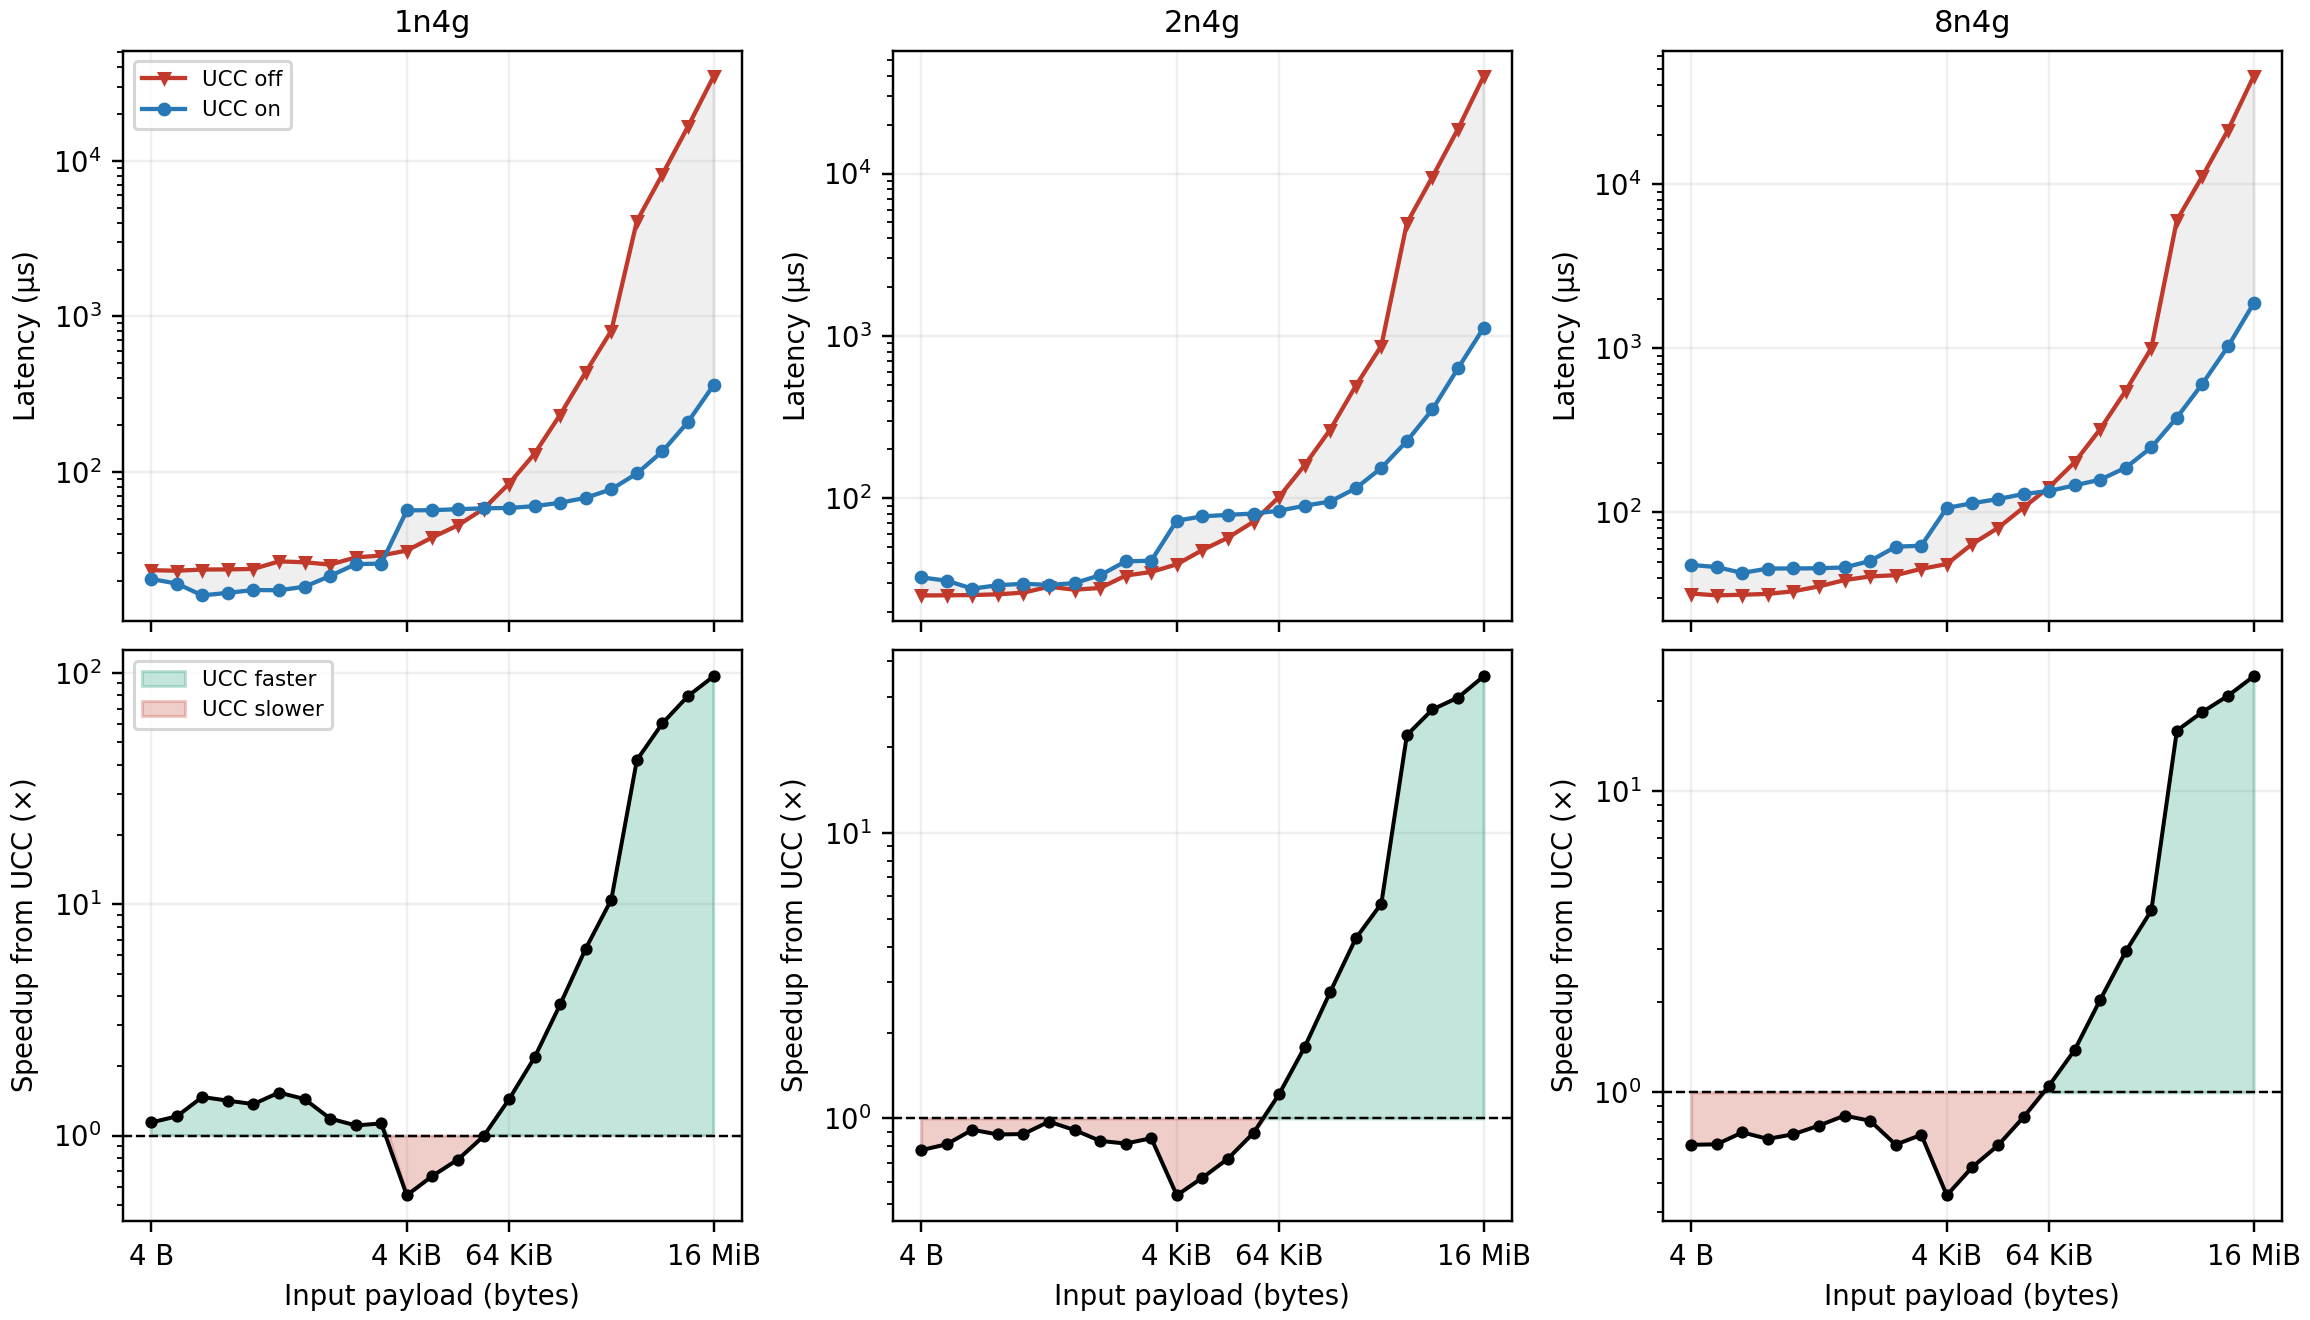
\includegraphics[width=\textwidth]{figures/results/ucc-ab-allreduce.png}
\caption[Effect of UCC on CUDA MPI \texttt{allreduce}]{Paired UCC \texttt{allreduce} control for CUDA MPI. Top: the measured cost of each configuration, so the divergence at large payloads is visible in absolute terms. Bottom: the resulting speedup, shaded green where UCC is faster and red where it is slower. Values are matched summary means; the SYCL MPI series tracks these curves closely and is omitted for legibility.}
\label{fig:m-ucc-allreduce}
\end{figure}

The discontinuity near 4\,KiB is consistent with the change, in the source of UCC's UCP transport layer, from a latency-oriented recursive k-nomial schedule to scatter-reduce/allgather k-nomial \cite{openucx_ucc_source_2026}. Source defaults explain a plausible mechanism, while forcing alternatives or recording the exact selected schedule would strengthen attribution for individual cells. The experiment uses one fixed UCC policy for the standalone allreduce sweep, so it does not claim a pointwise optimal configuration.

The single-rank \texttt{allreduce} control is anomalously slow for large buffers: the auxiliary UCC data report approximately 21\,ms at 16\,MiB, despite no inter-rank reduction. That cost is essentially unchanged by the UCC setting, at 21.9\,ms disabled against 21.4\,ms enabled, so it is not a collective-component effect. It is the same order of magnitude as the 34.9\,ms non-UCC four-rank result above, which is consistent with both being dominated by a local copy or reduction implementation rather than by transfer, though a one-rank control cannot separate those two by itself. It is excluded as a reference for network startup.

\subsection{All-to-All}

\texttt{alltoall} gives a clear example of runtime configuration changing the library ranking, with a UCC effect opposite to that of \texttt{allreduce}. Figure~\ref{fig:m-alltoall-backends} plots all seven stacks against bytes per peer, so the size axis is comparable across topologies. The default MPI latency changes sharply with GPU count and per-peer message size, while oneCCL/OSHMPI remains expensive because it stages the operands.

\begin{figure}[htbp]
\centering
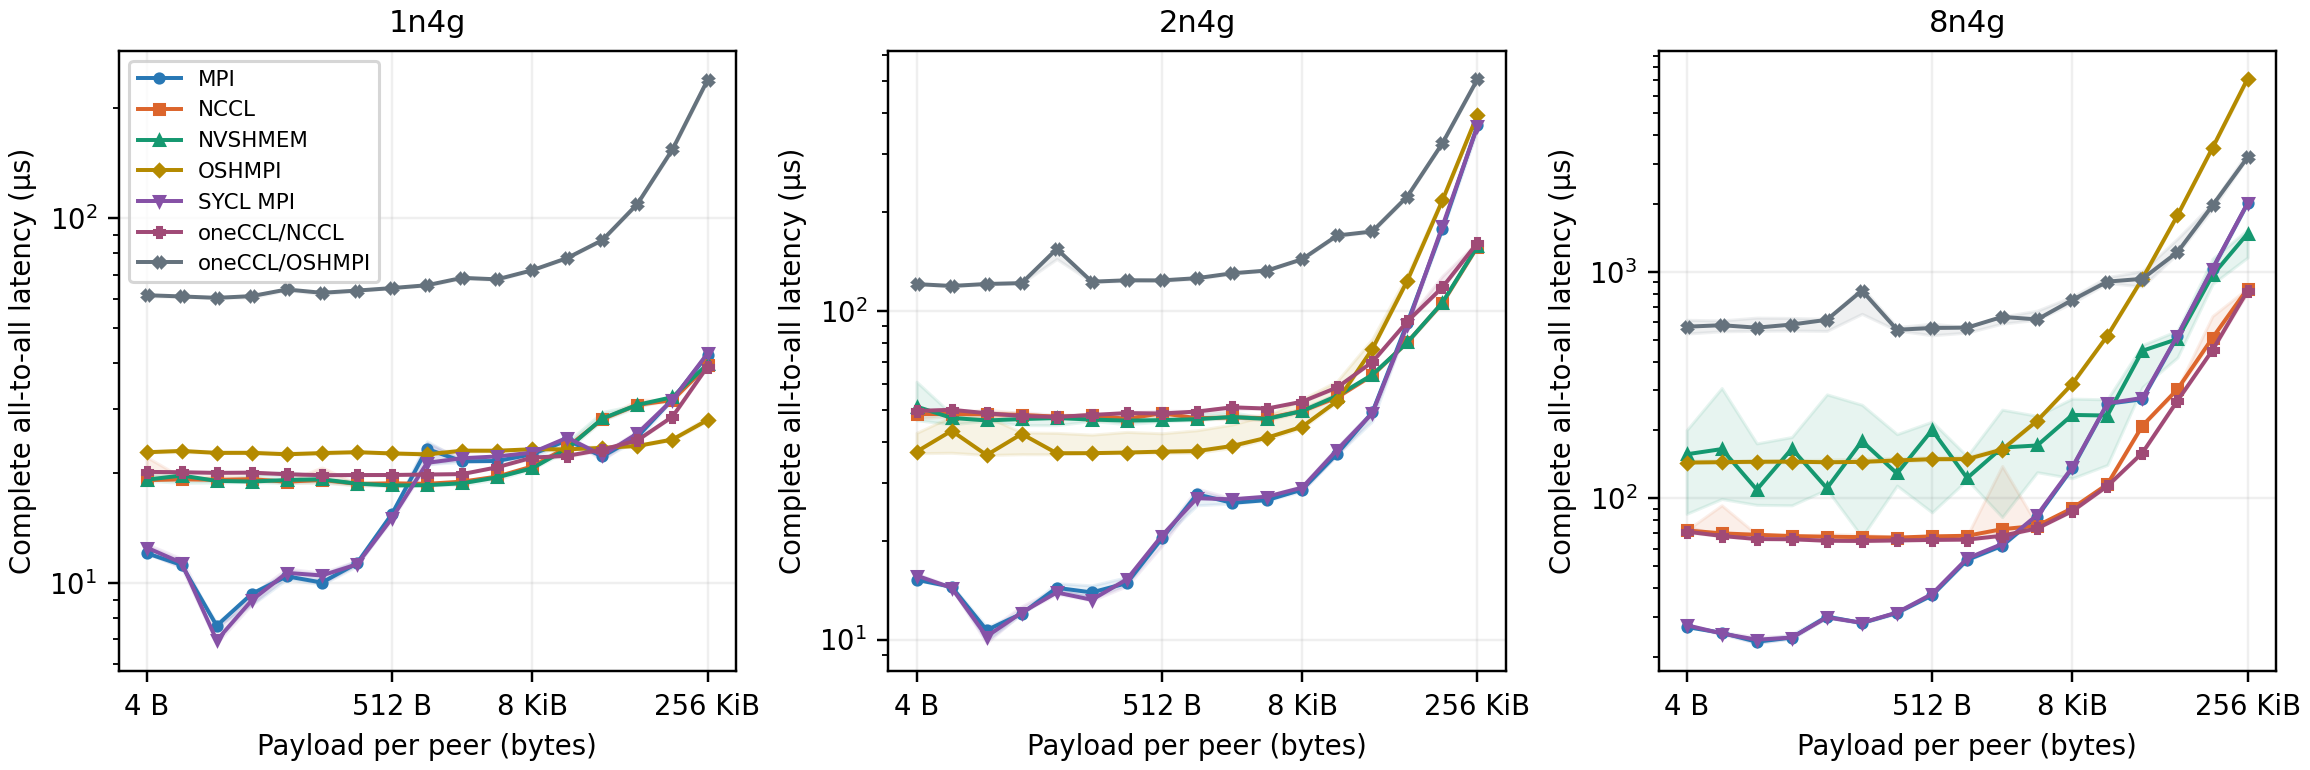
\includegraphics[width=\textwidth]{figures/results/alltoall-backends.png}
\caption[\texttt{alltoall} latency at representative topologies]{\texttt{alltoall} latency for all seven measured stacks at representative topologies. The horizontal axis is payload per peer; points are medians of allocation means and shading spans those means.}
\label{fig:m-alltoall-backends}
\end{figure}

At large payloads, NCCL-based implementations regain the advantage. Table~\ref{tab:m-alltoall-bandwidth} gives the endpoint at 256\,KiB per peer. Direct NCCL and oneCCL/NCCL are close enough that allocation variation matters when comparing them. Since the all-to-all archive combines measurement rounds, large performance differences are more reliable than small margins between backends.

\begin{table}[htbp]
\centering
\caption[\texttt{alltoall} aggregate bandwidth at 256\,KiB per peer]{\texttt{alltoall} aggregate bandwidth at 256\,KiB per peer, in GB/s. The numerator includes each rank's self block.}
\label{tab:m-alltoall-bandwidth}
\footnotesize
% Generated by tools/rebuild_main_evidence.py; include outside tabular.
\begin{tabular}{lrrrr}
\toprule
Topology & CUDA MPI & CUDA NCCL & CUDA NVSHMEM & oneCCL/NCCL\\
\midrule
\texttt{2n4g} & 5.7 & 13.4 & 13.3 & 13.0\\
\texttt{4n4g} & 4.4 & 10.3 & 8.2 & 10.5\\
\texttt{8n4g} & 4.2 & 10.0 & 5.7 & 10.2\\
\bottomrule
\end{tabular}

\end{table}

At the largest \texttt{8n4g} payload, direct NCCL and oneCCL/NCCL are within approximately 2\%. The combined adapter and SYCL overhead is much less visible here than in four-byte ping-pong. Together with the slower oneCCL/OSHMPI results, this shows why the adapter's design matters: asynchronous submission can retain the underlying library's throughput, while copying and blocking can consume its advantage.

\begin{keypoint}[All-to-all takeaway]
MPI needs appropriate algorithm selection to avoid the severe small-message slowdown and reaches 4.2\,GB/s at the \texttt{8n4g} bulk endpoint. Direct OSHMPI has the lowest throughput among the direct backends there. NVSHMEM keeps pace with NCCL within two nodes but falls to 5.7\,GB/s at \texttt{8n4g}. NCCL and oneCCL/NCCL lead at large payloads, at 10.0 and 10.2\,GB/s, and are within 2\% of each other. oneCCL/OSHMPI remains expensive because every block is staged through symmetric memory. SYCL MPI closely follows CUDA MPI overall.
\end{keypoint}

\subsubsection{Algorithm Selection and UCC}

Figure~\ref{fig:m-ucc-alltoall} shows the sharp change in MPI's small-message performance. At \texttt{8n4g}, disabling UCC gives 671--974\,$\mu$s for payloads at or below 256 bytes per peer, followed by an abrupt drop to 60\,$\mu$s at 512 bytes. With UCC enabled, the same small sizes take 24--31\,$\mu$s. The peak gain is 33.7 times at 128 bytes per peer. The benefit is concentrated at small messages and many GPUs: by 8\,KiB per peer the configurations agree within 2\%. At 256\,KiB per peer, UCC is slower, with speedup factors below one: 0.87 at \texttt{8n4g} and 0.56 at \texttt{2n4g}. Allreduce and all-to-all thus benefit from UCC at different message sizes, so one setting is not best for every operation.


\begin{figure}[htbp]
\centering
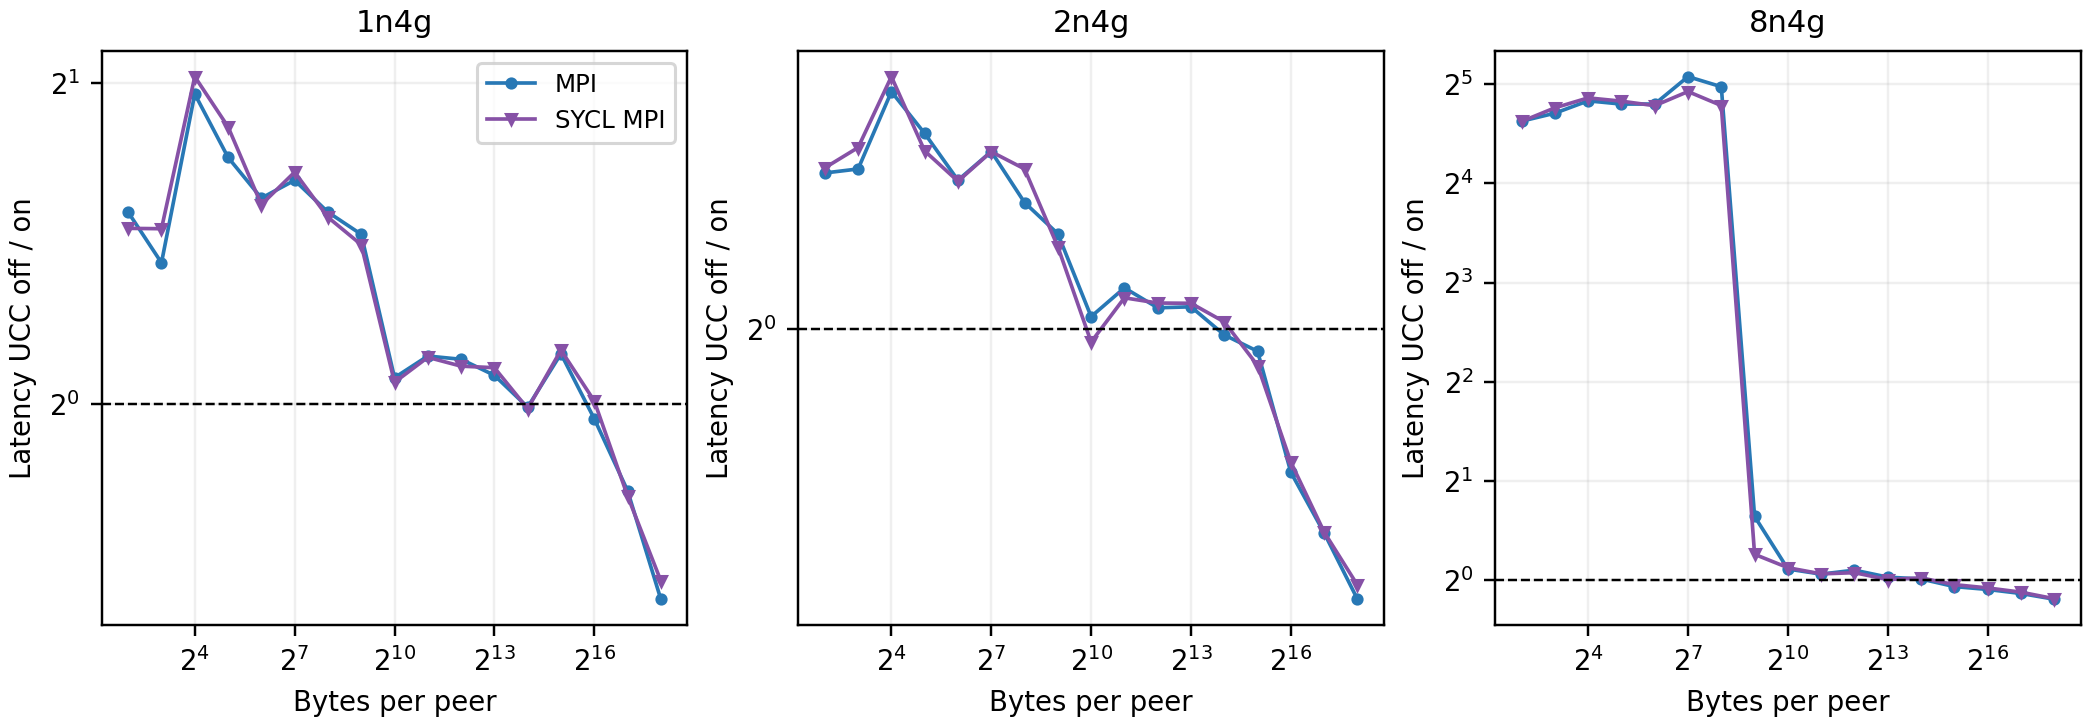
\includegraphics[width=\textwidth]{figures/results/ucc-ab-alltoall.png}
\caption[Effect of UCC on CUDA MPI \texttt{alltoall}]{Paired UCC \texttt{alltoall} control for CUDA MPI, against bytes per peer. Top: measured cost of each configuration; the flat non-UCC plateau below 512\,B per peer at \texttt{8n4g} is the modified-Bruck default. Bottom: the resulting speedup. The benefit is concentrated at small payloads and reverses at the largest ones, the opposite of the allreduce profile in Figure~\ref{fig:m-ucc-allreduce}.}
\label{fig:m-ucc-alltoall}
\end{figure}

Open MPI's tuned collective component lets each algorithm be selected explicitly. This control is enabled with \texttt{coll\_tuned\_use\_dynamic\_rules}. The \texttt{coll\_tuned\_alltoall\_algorithm} values 1, 2, 3, and 4 select linear, pairwise, modified Bruck, and synchronized-linear exchange, respectively. Each setting is measured in a separate run. Table~\ref{tab:m-alltoall-forced} shows the results at 16 ranks. Below 512 bytes per peer, the default closely matches modified Bruck, while forcing linear or synchronized-linear exchange avoids most of the penalty. This supports algorithm selection as an explanation for the slowdown, without attributing the full gain to UCC's network transport.

\begin{table}[htbp]
\centering
\caption[Open MPI all-to-all with forced algorithms]{Open MPI all-to-all with each algorithm forced explicitly, at 16 ranks with UCC disabled, in \,$\mu$s. Each column is a separate run with \texttt{coll\_tuned\_alltoall\_algorithm} set to that algorithm; the last column lets Open MPI choose. Values are retained from the configuration-analysis record.}
\label{tab:m-alltoall-forced}
\scriptsize
\begin{tabular}{rrrrrr}
\toprule
B/peer & Linear & Pairwise & Modified Bruck & Linear sync & Default\\
\midrule
4 & 25.7 & 64.8 & 340.0 & 29.9 & 342.3\\
16 & 22.1 & 58.1 & 341.4 & 24.5 & 341.2\\
256 & 27.9 & 72.4 & 421.2 & 29.6 & 420.0\\
512 & 31.7 & 79.6 & 429.2 & 34.9 & 38.8\\
\bottomrule
\end{tabular}
\end{table}

Modified Bruck reduces communication rounds by forwarding data, but the Open MPI implementation also rotates buffers, constructs indexed datatypes, and copies noncontiguous blocks \cite{bruck_alltoall_1997,openmpi_alltoall_source_2026}. Those local operations can be expensive on GPU-resident buffers. The UCC dispatch trace identifies its UCP transport layer, whose CUDA default uses contiguous peer slices and nonblocking tagged communication \cite{venkata_ucc_2024,openucx_ucc_source_2026}. This explains the structural difference; it does not replace a profile of individual copy costs.

\subsection{Scale-Up and Scale-Out}\label{sec:micro-scaling}

The topology sweep separates adding GPUs within a node from adding nodes. \emph{Scaling up} keeps transfers within NVLink; \emph{scaling out} puts some traffic on InfiniBand. A stack can perform well in one case and poorly in the other. For the steady-state halo at a 16\,MiB aggregate payload, OSHMPI reaches 325\,GB/s and CUDA MPI 280\,GB/s at \texttt{1n4g}. On \texttt{2n1g}, every stack reaches only 20--24\,GB/s. The much lower network bandwidth is important here, although topology can also change the selected algorithms and progress mechanisms. With four GPUs per node, the rate stays essentially flat as nodes are added: NVSHMEM holds 41.1, 40.9, and 40.6\,GB/s at \texttt{2n4g}, \texttt{4n4g}, and \texttt{8n4g}, and CUDA MPI holds 33.9--36.5\,GB/s over the same range. This plateau is consistent with a limit on how much traffic each node can inject.

\texttt{allreduce} behaves differently. At 16\,MiB, NCCL takes 1557\,$\mu$s on \texttt{2n1g}, with only two GPUs, but 1104\,$\mu$s on \texttt{8n4g}, with 32 GPUs. A hierarchical reduction can combine work over NVLink before sending data across InfiniBand, reducing the network payload. This helps explain why NCCL-based implementations pull away from MPI when each node holds four GPUs: NCCL takes 567\,$\mu$s against 1118\,$\mu$s at \texttt{2n4g}, and 1104\,$\mu$s against 1879\,$\mu$s at \texttt{8n4g}. A four-byte scalar offers little opportunity to reduce the network payload. Its allreduce latency instead rises with GPU count, from roughly 18--20\,$\mu$s at \texttt{1n4g} to 46--49\,$\mu$s at \texttt{8n4g} for every stack except NVSHMEM, which reaches 88\,$\mu$s.

These examples show why GPU count alone is insufficient for stack selection. A result measured over NVLink need not hold across a network, while multiple GPUs per node can enable hierarchical algorithms that improve network efficiency. The remaining topology panels are in Appendix~\ref{app:complete-results}.

\subsection{SYCL Portability}\label{sec:sycl-portability}

Two paired comparisons assess the effect of using SYCL. SYCL MPI and CUDA MPI use the same communication library with different compute interfaces. Comparing oneCCL/NCCL with direct NCCL also includes an adapter. Table~\ref{tab:m-sycl-portability} summarizes the per-cell timing ratios for each pattern, showing the median and maximum SYCL MPI ratios and the median oneCCL/NCCL ratio.

\begin{table}[htbp]
\centering
\caption[SYCL relative to CUDA by pattern]{SYCL relative to CUDA over all measured cells of each pattern, as median and maximum of the per-cell ratio. Values above one favor CUDA.}
\label{tab:m-sycl-portability}
\footnotesize
\begin{tabularx}{\textwidth}{lYrrr}
\toprule
Pattern & Cells & SYCL/CUDA median & SYCL/CUDA max & oneCCL/NCCL median\\
\midrule
\texttt{pingpong} & 46 & $1.01$ & $1.84$ & $1.10$\\
\texttt{halo\_1d}, isolated & 126 & $1.02$ & $1.19$ & $1.32$\\
\texttt{halo\_1d}, steady & 126 & $1.01$ & $1.07$ & $1.13$\\
\texttt{allreduce} & 161 & $1.00$ & $1.06$ & $1.02$\\
\texttt{alltoall} & 119 & $1.01$ & $1.06$ & $1.02$\\
\texttt{moe} & 21 & $1.00$ & $1.08$ & $1.02$\\
\midrule
\texttt{cg\_step} & 30 & $1.34$ & $1.51$ & $1.57$\\
\bottomrule
\end{tabularx}
\end{table}

For the five patterns that time communication alone, SYCL MPI costs about 1\% more than CUDA MPI at the median. The largest deviations occur in ping-pong, reaching $1.84\times$ at large messages; isolated halo exchanges reach $1.19\times$, while the other communication-only rows stay within 8\%. Small-message ping-pong timings remain close. Overall, the median overhead is small when both implementations use the same transfers, transport, and completion requirements, with changes limited to host submission and buffer allocation.

The \texttt{cg\_step} benchmark has a larger median gap, at $1.34\times$ over its multi-rank cells, and is the only pattern that includes computation. Communication-only timings are much closer, suggesting that the benchmark's kernels and host coordination contribute to the additional cost. The solver comparison in Section~\ref{sec:acg-sycl} tests whether a SYCL application shows a similar difference.

The oneCCL/NCCL column behaves differently, because it adds an adapter to the compute-interface change. It is within 2\% of direct NCCL for the three collective patterns, but reaches $1.32\times$ for the isolated halo and $1.10\times$ for ping-pong, the two cases where submission cost is exposed rather than amortized. A common interface is therefore inexpensive where the operation is large enough to hide its submission, and visible where it is not.

These primitive results leave several plausible candidates: MPI for startup-sensitive transfers, persistent NVSHMEM for large repeated halos, and NCCL-based paths for bulk collectives. The next question is whether composing operations preserves those advantages.

\section{Mixture-of-Experts Dispatch and Combine}\label{sec:moe-results}

The two application microbenchmarks address different threats to the primitive rankings. This section covers \texttt{moe}, which keeps the redistribution operation but abandons the assumption that every peer receives the same number of bytes. Section~\ref{sec:cg-step-results} then covers \texttt{cg\_step}, the level that Section~\ref{sec:acg-results} pairs with the solver.

\subsection{Routing Cases}

The \texttt{moe} archive is complete for the six declared stacks across all seven topologies and all three routing cases, with five allocations of three trials per cell. Total useful volume is held fixed at 32\,MiB per rank for dispatch and combine together, so a difference between routing cases is a difference in distribution, not in bytes moved.

Figure~\ref{fig:m-moe-scaling} reproduces the interconnect boundary identified in Section~\ref{sec:micro-scaling} and adds a second, routing-dependent one. Under \texttt{uniform} routing the intra-node curves fall from \texttt{1n2g} to \texttt{1n4g}, because a fixed per-rank token count is divided among more experts while NVLink absorbs the traffic: CUDA MPI improves from 253\,$\mu$s to 179\,$\mu$s. Crossing to \texttt{2n1g} costs roughly an order of magnitude, to 1743\,$\mu$s, and beyond that the stacks separate. NCCL and oneCCL/NCCL rise to only about 3.0\,ms at \texttt{8n4g}, while the MPI paths reach about 6.0\,ms and OSHMPI 10.4\,ms.

\begin{figure}[htbp]
\centering
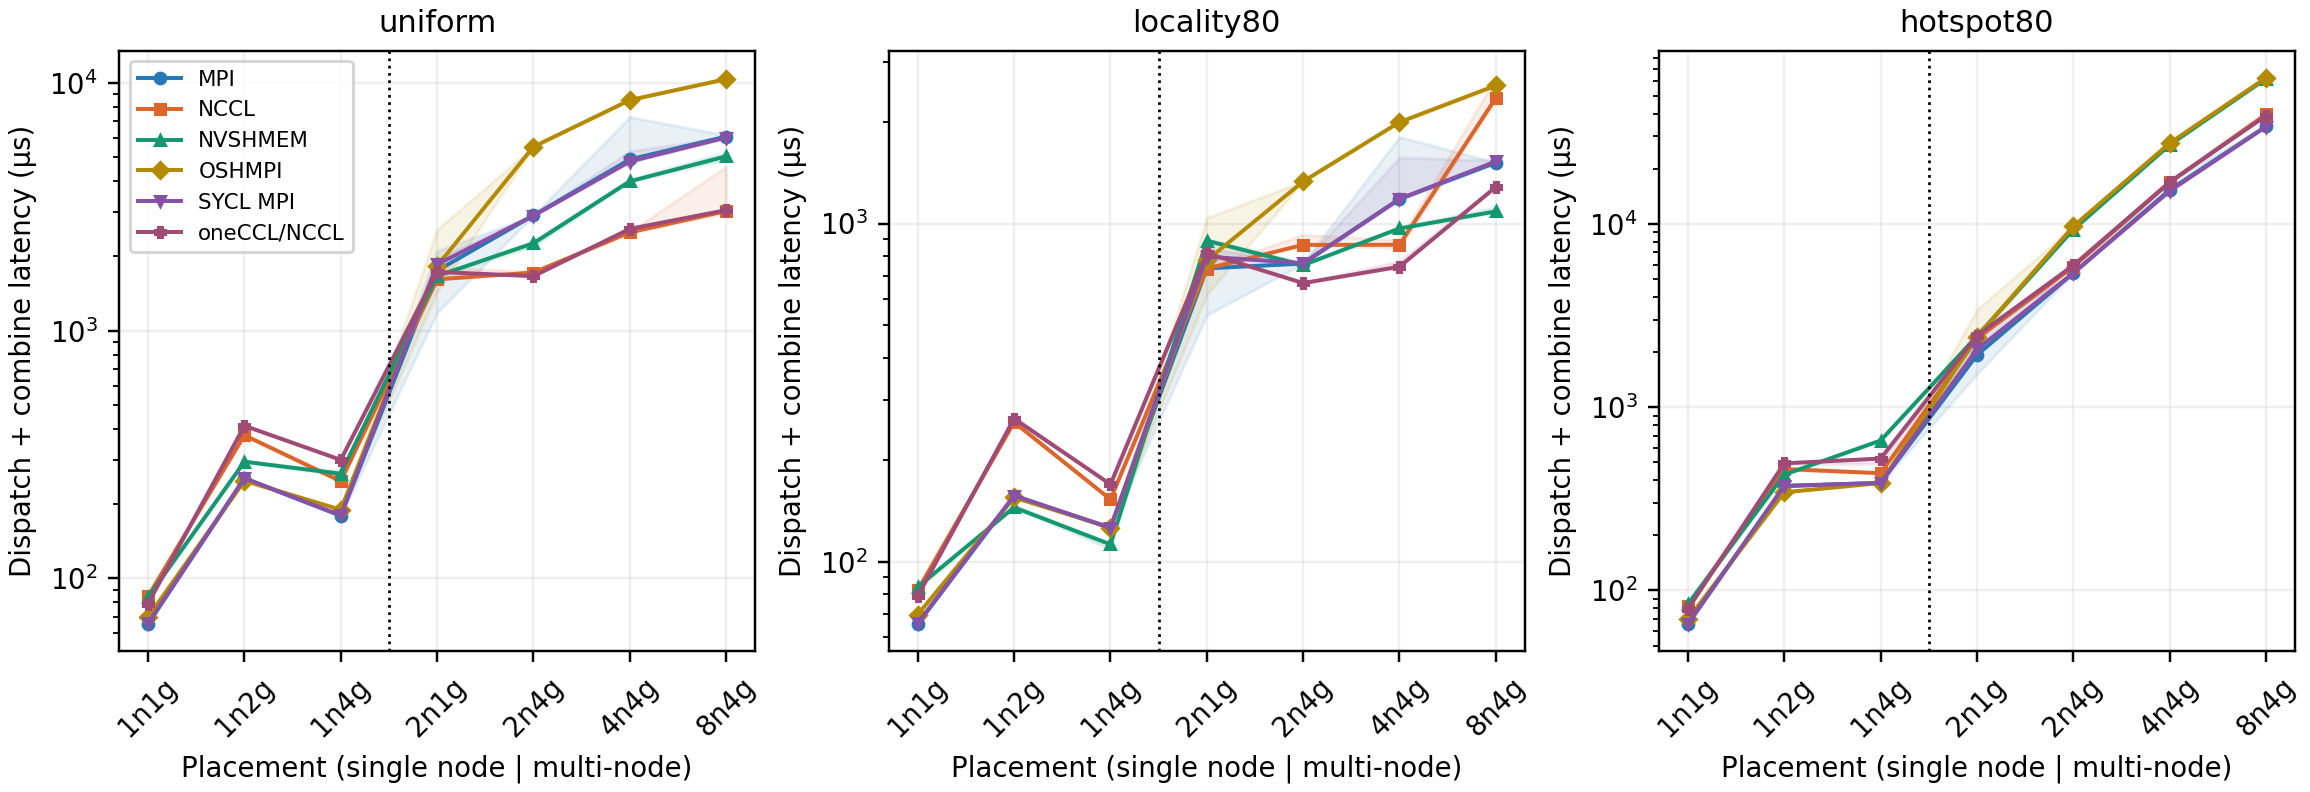
\includegraphics[width=\textwidth]{figures/results/moe-routing-scaling.png}
\caption[\texttt{moe} latency by topology and routing case]{\texttt{moe} dispatch-and-combine latency for the six measured stacks at every topology, under the three routing cases. Points are medians of five allocation means and shading spans those means. The dotted line separates intra-node NVLink topologies from those crossing InfiniBand. At \texttt{1n1g} all three cases degenerate to a local copy.}
\label{fig:m-moe-scaling}
\end{figure}

Table~\ref{tab:m-moe} gives the endpoints. The intra-node columns are tightly grouped: at \texttt{1n4g} under \texttt{uniform} routing the six stacks span 179--301\,$\mu$s. The multi-node columns are not: the same six stacks span 3038--10350\,$\mu$s. Selecting a stack on the intra-node result alone would be uninformative here, because the measurement that separates the candidates is the one that crosses the fabric.

\begin{table}[htbp]
\centering
\caption[\texttt{moe} dispatch-and-combine latency]{\texttt{moe} dispatch-and-combine latency in \,$\mu$s, medians of allocation means, contrasting the largest intra-node topology with the largest multi-node topology for each routing case.}
\label{tab:m-moe}
\footnotesize
% Generated by tools/import_moe_evidence.py; include outside tabular.
\begin{tabular}{lrrrrrr}
\toprule
Stack & Uni.\ \texttt{1n4g} & Uni.\ \texttt{8n4g} & Loc.\ \texttt{1n4g} & Loc.\ \texttt{8n4g} & Hot.\ \texttt{1n4g} & Hot.\ \texttt{8n4g}\\
\midrule
MPI & 179 & 6071 & 126 & 1513 & 386 & 34028\\
SYCL MPI & 180 & 6013 & 126 & 1527 & 386 & 33945\\
NCCL & 247 & 3038 & 153 & 2352 & 436 & 39617\\
NVSHMEM & 264 & 5050 & 112 & 1086 & 658 & 62007\\
OSHMPI & 189 & 10350 & 126 & 2561 & 386 & 62686\\
oneCCL/NCCL & 301 & 3063 & 169 & 1283 & 524 & 38924\\
\bottomrule
\end{tabular}

\end{table}

\subsection{Backend Ranking}

Figure~\ref{fig:m-moe-sensitivity} shows how routing changes the ranking at \texttt{8n4g}. No stack is faster than CUDA MPI in all three cases. Three of the five alternatives switch from faster to slower than MPI as routing changes.

Under \texttt{uniform} routing, the two NCCL-based implementations are fastest, taking approximately half of CUDA MPI's time. Under \texttt{locality80}, direct NCCL instead takes 1.55 times as long as CUDA MPI. With 80\% of tokens staying local, the remote exchanges are smaller and irregular. This reversal is consistent with submission overhead becoming more important when it is spread over less transferred data.

NVSHMEM benefits from locality: its time relative to MPI falls from 0.83 under \texttt{uniform} to 0.72 under \texttt{locality80}, the lowest measured ratio. Its per-destination puts can handle the small, uneven blocks directly, which may help explain the different response to routing.

\begin{figure}[htbp]
\centering
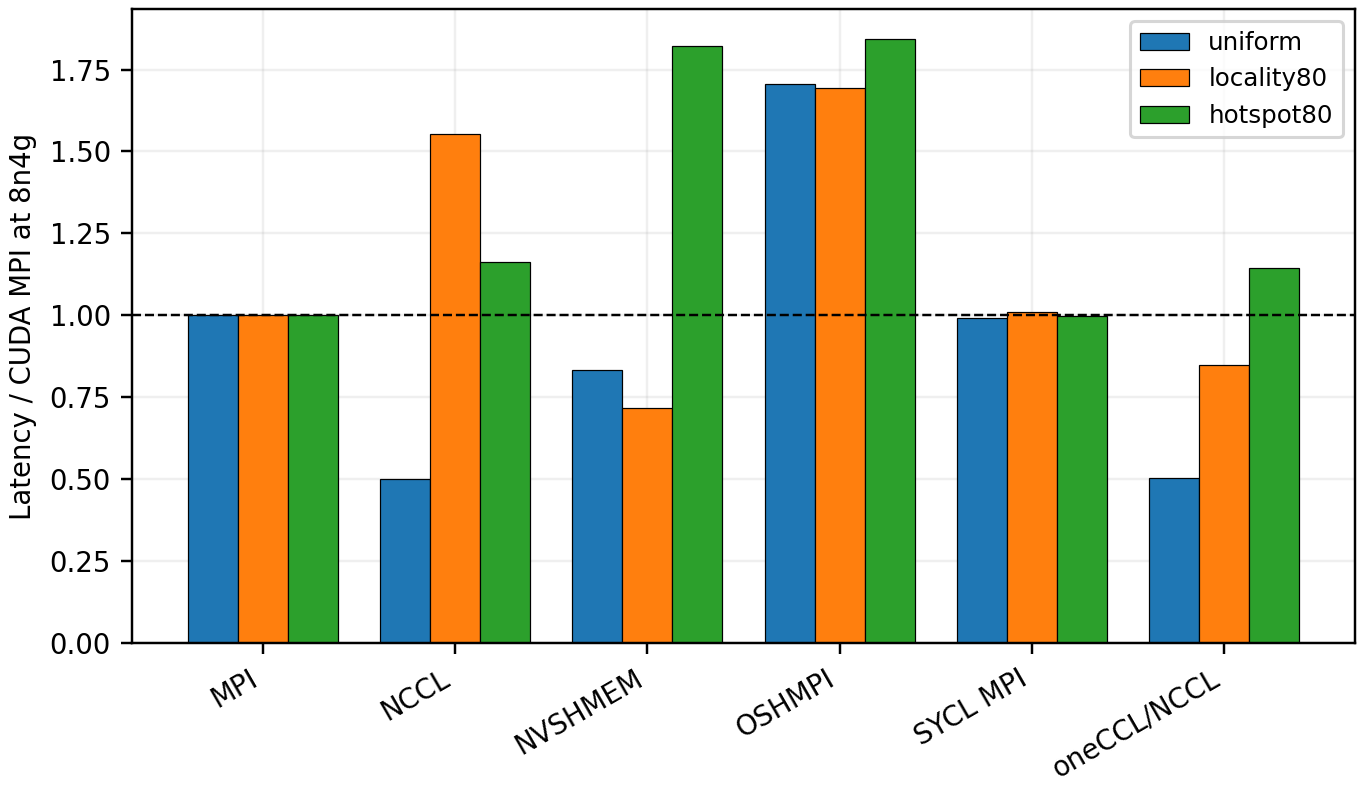
\includegraphics[width=0.78\textwidth]{figures/results/moe-routing-sensitivity.png}
\caption[\texttt{moe} latency at \texttt{8n4g} relative to CUDA MPI]{\texttt{moe} latency at \texttt{8n4g} relative to CUDA MPI at the same topology and routing case. Bars below one favor the compared stack. No stack is below one in all three cases.}
\label{fig:m-moe-sensitivity}
\end{figure}

The \texttt{hotspot80} case concentrates 80\% of tokens on rank 0, slowing every stack at \texttt{8n4g}. CUDA MPI takes 34.0\,ms, while NVSHMEM and OSHMPI take 62.0 and 62.7\,ms, about 1.8 times as long. The \texttt{alltoallv} implementations can schedule the uneven exchange as a collective. The SHMEM implementations issue puts in the order ranks produce them, without a collective algorithm to reorganize traffic arriving at the same destination. This difference may contribute to the slowdown, but the measurements do not separate scheduling costs from congestion at the receiving NIC.

OSHMPI is the one stack that is slower than CUDA MPI in every routing case at \texttt{8n4g}, by 1.70 to 1.84 times, despite matching MPI within one node at \texttt{1n4g} under two of the three cases. Its per-phase quiet, device synchronization, and barrier are inexpensive when every put lands on NVLink and expensive once each of them must complete across the fabric.

Two qualifications bound these results. \texttt{moe} keeps UCC disabled and uses the variable-count Open MPI path, so the MPI series is one fixed configuration rather than a tuned result, and the all-to-all tuning of Section~\ref{sec:micro-results} does not transfer to it untested. Second, the reported volume is useful application bytes including tokens that never leave their source rank, so the \texttt{locality80} latencies correspond to much less traffic than their byte count suggests; they are comparable across stacks, not convertible into a link rate.

\subsection{Comparison with All-to-All}

The standalone \texttt{alltoall} sweep of Section~\ref{sec:micro-results} sends equal blocks to every peer and favors NCCL-based implementations at large payloads. The \texttt{moe} comparison shows why that result cannot be applied to every redistribution: at the same topology and fixed useful volume, routing-dependent exchanges reverse the ranking in two of three cases. Message-size distribution matters as well as total volume.

Section~\ref{sec:cg-step-results} finds a related limitation in \texttt{cg\_step}: matching the operation and payload is insufficient when the submission sequence changes. Here the important change is routing. Both examples show which application details a benchmark must reproduce before its ranking can guide stack selection.

\begin{keypoint}[MoE takeaway]
MPI provides a competitive reference across all three routing cases, although it is never fastest. OSHMPI is 1.70--1.84 times slower than MPI at \texttt{8n4g}, despite matching it within a node in two cases. NVSHMEM is fastest under locality-biased routing at \texttt{8n4g}, taking 0.72 of MPI's time, but both put-based implementations suffer under a hotspot. NCCL is fastest under uniform routing and becomes 1.55 times slower than MPI when most tokens stay local. oneCCL/NCCL follows direct NCCL under uniform routing, at about half of MPI's time. SYCL MPI tracks CUDA MPI. The best choice depends on where the tokens go.
\end{keypoint}

\section{Simplified CG Iteration Benchmark}\label{sec:cg-step-results}

\subsection{Step Time}

The \texttt{cg\_step} comparison covers six multi-rank topologies, five global grid sides, and six backends, with nine successful trials per cell. Single-GPU runs are excluded because they perform no inter-rank communication. The benchmark combines a halo, stencil, and reductions, but stops before using the reduced scalars in a subsequent GPU update. Table~\ref{tab:m-cg-step} lists the lowest allocation-median times for this sequence. OSHMPI leads 25 of the 30 cells, including all multi-node topologies; NCCL leads the remaining five intra-node cells.

\begin{table}[htbp]
\centering
\caption[Lowest \texttt{cg\_step} time by topology and grid side]{Lowest allocation-median \texttt{cg\_step} time by topology and global grid side. This is a point-estimate ranking for the synthetic sequence, not a significance test or a solver-ready ranking.}
\label{tab:m-cg-step}
\footnotesize
% Generated by tools/rebuild_main_evidence.py; include outside tabular.
\begin{tabular}{lccccc}
\toprule
Topology & 512 & 1024 & 2048 & 4096 & 8192\\
\midrule
\texttt{1n2g} & NCCL & NCCL & NCCL & OSHMPI & OSHMPI\\
\texttt{1n4g} & OSHMPI & NCCL & NCCL & OSHMPI & OSHMPI\\
\texttt{2n1g} & OSHMPI & OSHMPI & OSHMPI & OSHMPI & OSHMPI\\
\texttt{2n4g} & OSHMPI & OSHMPI & OSHMPI & OSHMPI & OSHMPI\\
\texttt{4n4g} & OSHMPI & OSHMPI & OSHMPI & OSHMPI & OSHMPI\\
\texttt{8n4g} & OSHMPI & OSHMPI & OSHMPI & OSHMPI & OSHMPI\\
\bottomrule
\end{tabular}

\end{table}

Figure~\ref{fig:m-cg-relative} shows why the margin matters. The direct CUDA paths approach one another as the local work per GPU grows. At larger rank counts, communication and orchestration remain visible, and NVSHMEM exhibits substantial allocation variation. Some intra-node NCCL and OSHMPI estimates are close enough that assigning a categorical winner overstates the evidence.

\begin{figure}[htbp]
\centering
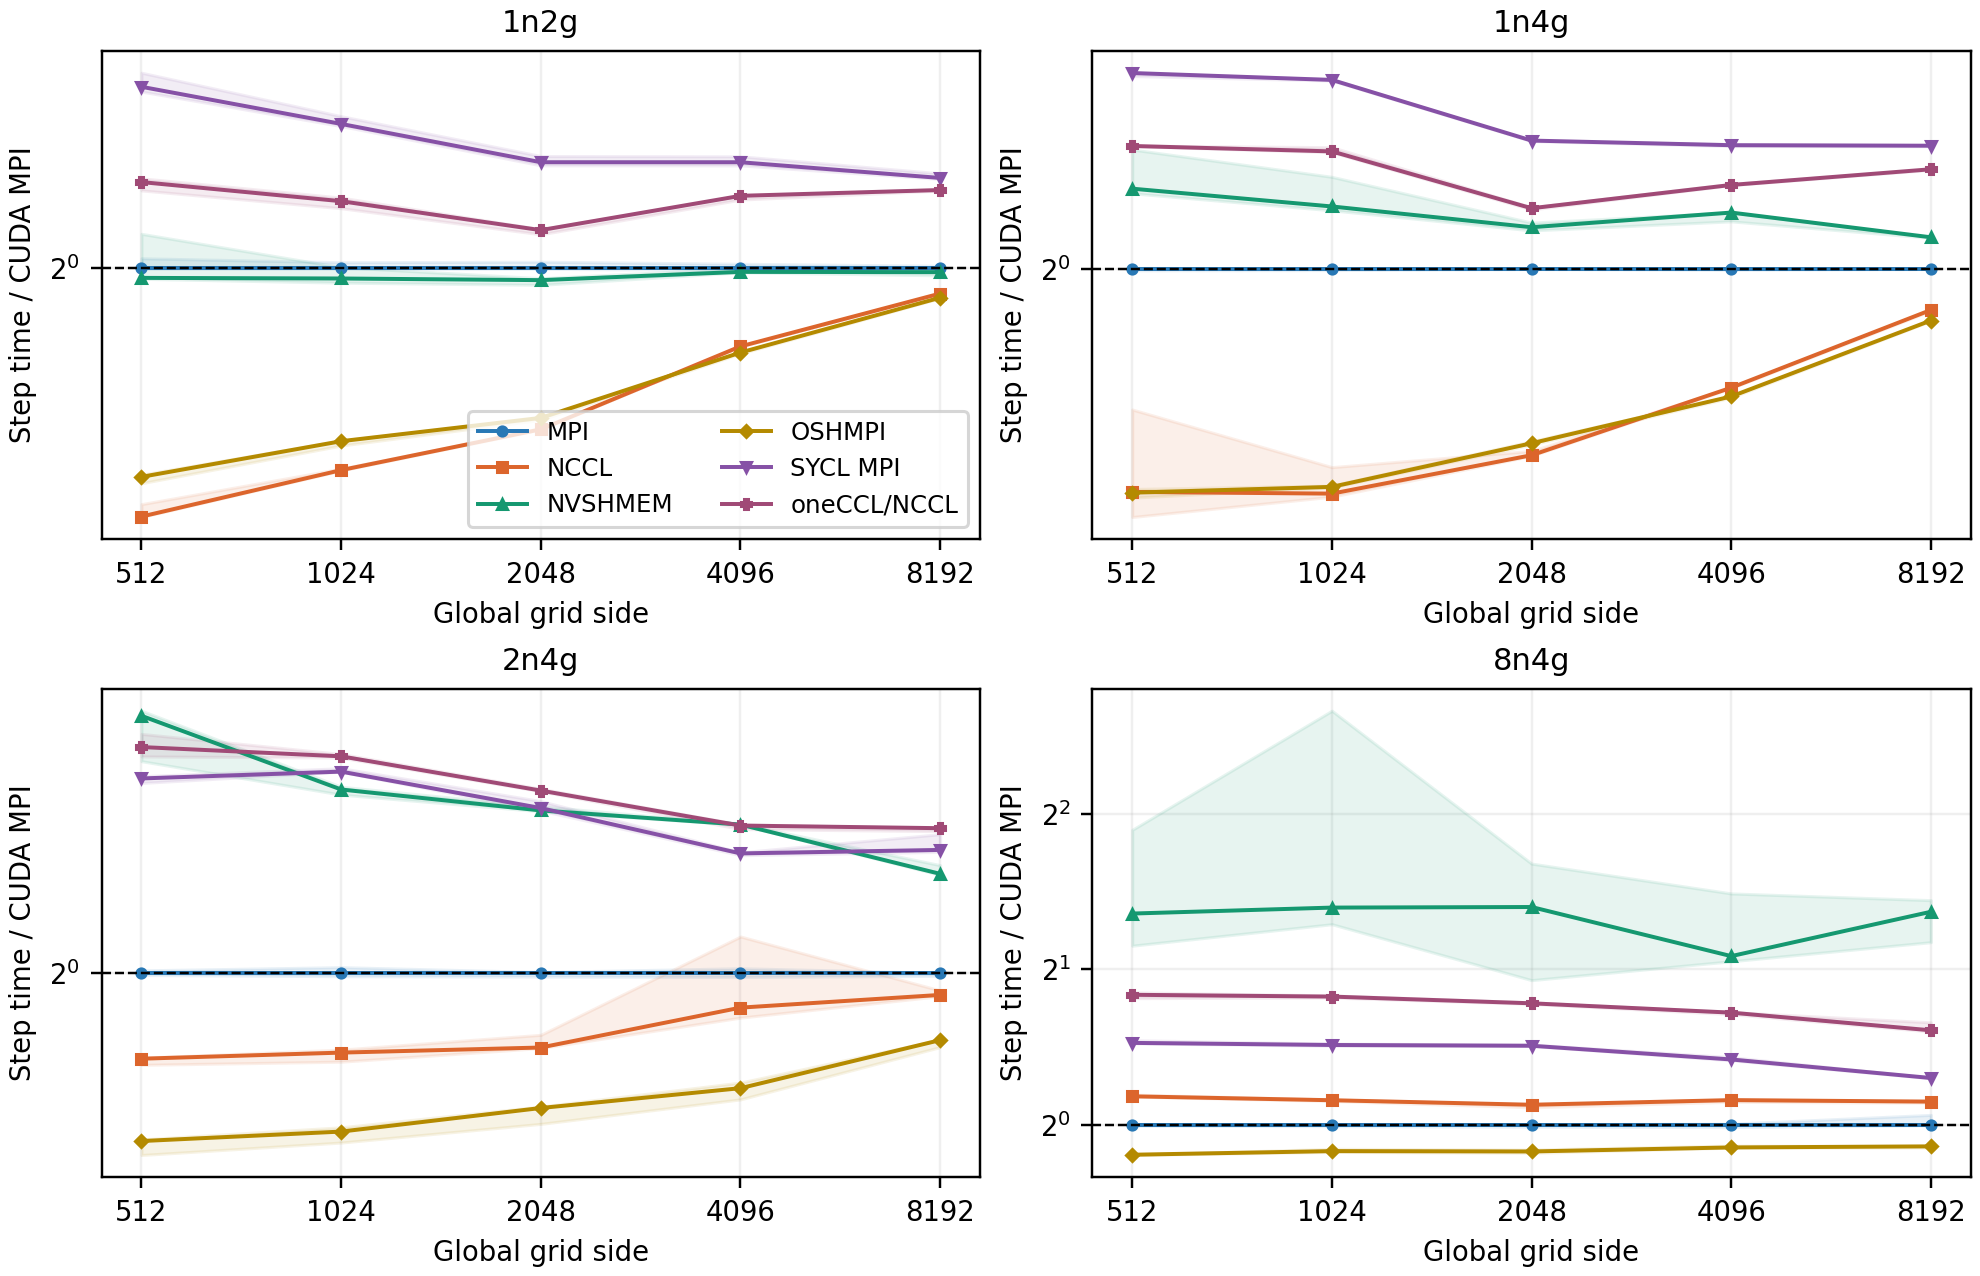
\includegraphics[width=\textwidth]{figures/results/cg-step-relative.png}
\caption[\texttt{cg\_step} time relative to CUDA MPI]{\texttt{cg\_step} time relative to CUDA MPI at the same global grid side and topology. Centers are allocation medians; bands are allocation ranges divided by the fixed reference median, not confidence intervals for the ratio. Values below one favor the compared stack. Only multi-rank topologies are shown: at \texttt{1n1g} no inter-rank communication occurs.}
\label{fig:m-cg-relative}
\end{figure}

The measured OSHMPI implementation leaves the reduction result in host memory. It avoids copying that result back to the GPU and waiting for it before the next computation, both of which a solver would require. Its low synthetic-step time therefore needs application-level validation before it can justify choosing OSHMPI for CG reductions.

\subsection{Device-Initiated Step}\label{sec:cg-device}

The device-initiated implementation of \texttt{cg\_step} issues the halo exchange and both scalar reductions from inside the kernel, so it is the benchmark-level counterpart of the monolithic device solver. It was measured over every topology and seven grid sides from 256 to 16\,384, with three allocations of three trials per cell, except at \texttt{8n4g}, where the smallest and largest sides are missing. It reports no phase timers, so it appears in step time only and not in the phase breakdown below.

Its result depends on both axes at once. Against its own host counterpart it is consistently better once communication crosses the fabric: at \texttt{8n4g} it takes 0.63 of host NVSHMEM's step time at side 512 and 0.52 at side 8192. Against the best host stack of each cell, however, it leads only where the problem is small and the GPU count low, at 0.69 of the fastest host time on \texttt{1n2g} and 0.82 on \texttt{1n4g} at side 512. It falls behind from eight GPUs upward at that side, at 1.12 to 1.25, and behind everywhere at side 8192, where its \texttt{1n2g} step costs 1.84 times the fastest host stack. Device initiation therefore helps this step where per-GPU work is small enough for launch and synchronization costs to dominate, and does not compensate for a slower local execution once the stencil and dot products grow.

Figure~\ref{fig:m-cg-device-step} contrasts the two problem sizes. At side 512, the device implementation is fastest on \texttt{1n2g}, but its time then rises and crosses the MPI and OSHMPI curves at \texttt{2n4g}. Dividing only 512 columns across more GPUs leaves less local computation while the halo and two reductions still have to finish before the next step. At side 8192, the device curve decreases as GPUs are added and follows the host curves more closely in shape, even where its absolute time is higher. The next comparison asks whether that scaling shape resembles the solver's.

\begin{figure}[!htbp]
\centering
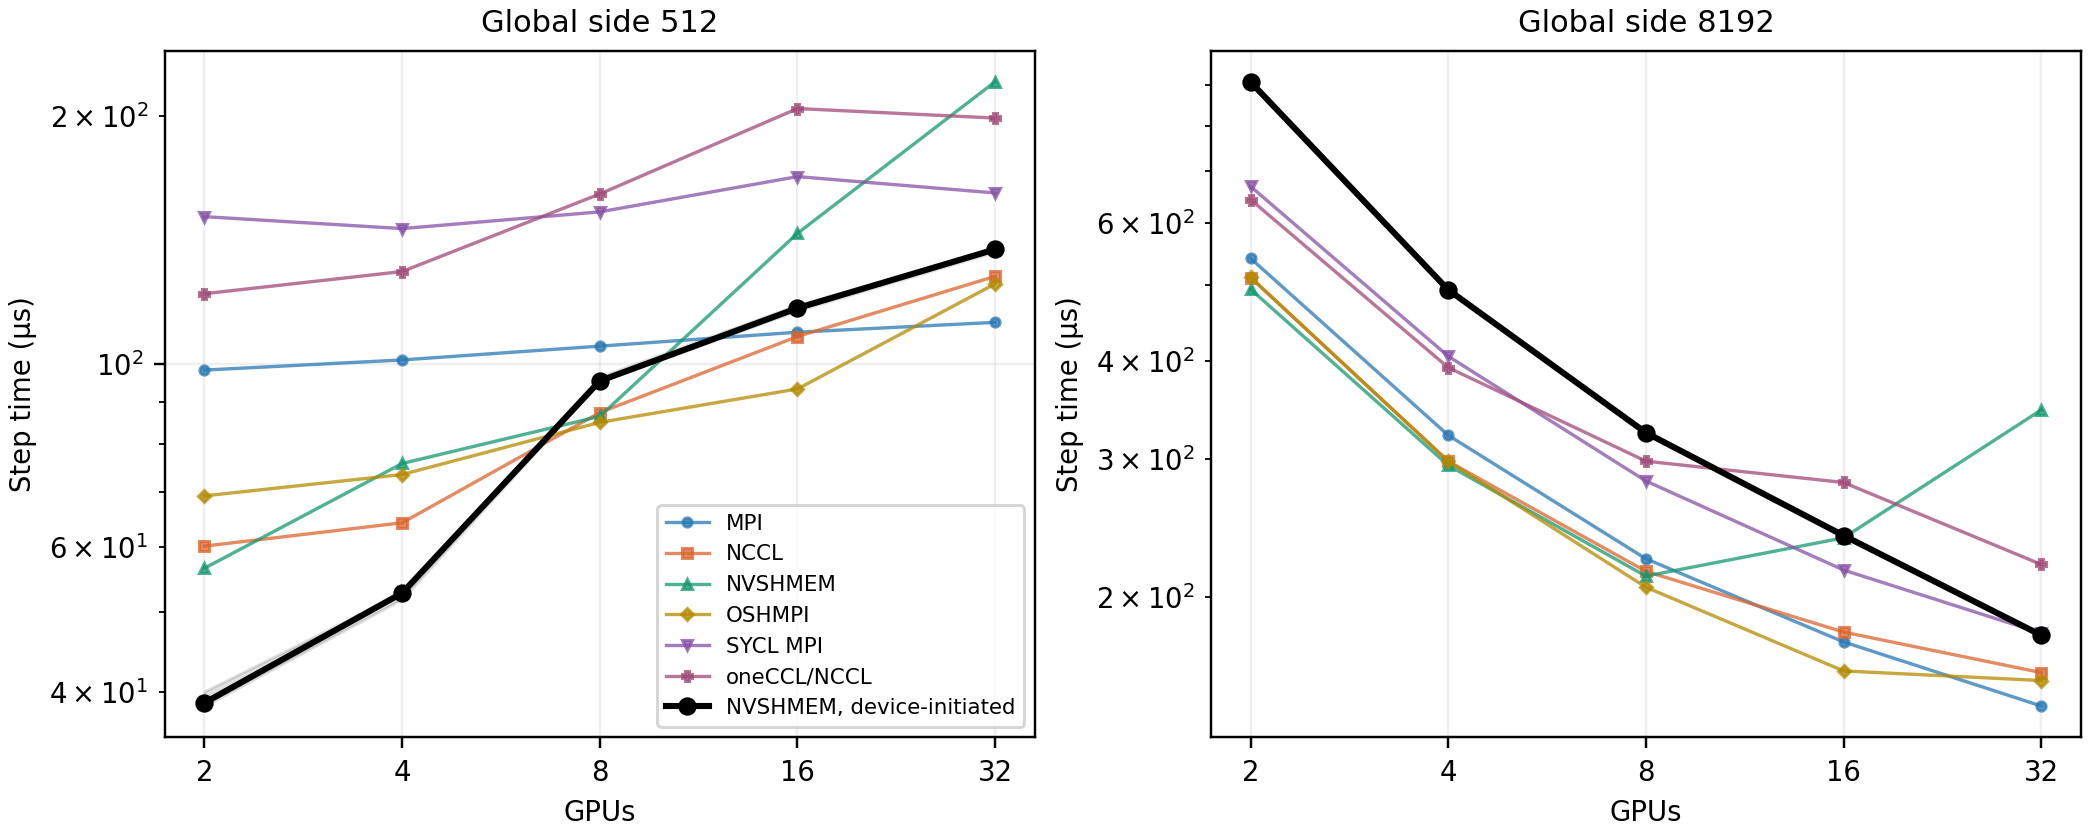
\includegraphics[width=\textwidth]{figures/results/cg-device-step.png}
\caption[Device-initiated versus host-initiated \texttt{cg\_step}]{Step time of the device-initiated \texttt{cg\_step} against the host implementations at the smallest and a large grid side. All series come from the same later snapshot, in which the host implementations were measured with one allocation and therefore carry no range; the shaded band is the allocation range of the device implementation.}
\label{fig:m-cg-device-step}
\end{figure}


\subsection{Phase Breakdown}

Table~\ref{tab:m-cg-phases} uses the separate synchronized phase pass at \texttt{4n4g}, side 512. The OSHMPI reduction phase is smaller than the corresponding MPI and NCCL phases, while NVSHMEM's halo and reduction costs contribute to its larger total. The SYCL paths also expose additional computation and runtime costs.

\begin{table}[htbp]
\centering
\caption[\texttt{cg\_step} phase costs on \texttt{4n4g}]{Archived mean \texttt{cg\_step} phase costs on \texttt{4n4g}, side 512, in \,$\mu$s. Step is the unsplit mean; gap is phase sum minus step.}
\label{tab:m-cg-phases}
\scriptsize
% Generated by tools/rebuild_main_evidence.py; include outside tabular.
\begin{tabular}{lrrrrrrr}
\toprule
Backend & Pack & Halo & Compute & Reduce & Sum & Step & Gap\\
\midrule
MPI & 13.3 & 23.7 & 24.6 & 58.7 & 120.3 & 111.3 & 9.0\\
NCCL & 28.5 & 38.6 & 23.0 & 76.3 & 166.3 & 107.7 & 58.6\\
NVSHMEM & 14.3 & 77.6 & 35.6 & 125.4 & 252.8 & 215.5 & 37.3\\
OSHMPI & 13.5 & 25.3 & 24.4 & 37.7 & 100.9 & 88.9 & 12.0\\
SYCL MPI & 11.3 & 25.2 & 67.6 & 62.3 & 166.4 & 164.0 & 2.4\\
oneCCL/NCCL & 11.7 & 48.8 & 45.7 & 107.4 & 213.6 & 183.0 & 30.6\\
\bottomrule
\end{tabular}

\end{table}

For NCCL, the phase sum is approximately 166.3\,$\mu$s and the unsplit mean 107.7\,$\mu$s. Their 58.6\,$\mu$s difference is about 35\% of the phase sum, or 54\% of the unsplit time. The denominator changes the percentage. More importantly, the gap includes synchronization introduced by instrumentation and variation between passes; it cannot be reported as a measured overlap fraction.

\subsection{Scalar Reduction Placement}

The auxiliary OSHMPI placement control compares host-staged reductions with CUDA symmetric operands and UCC enabled (Table~\ref{tab:m-oshmpi-reduce-placement}). It reports a larger reduction cost in the device/UCC arm and a concurrent increase in computation time. These are relative effects from the separate control record, not phase values substituted into the reconciled main sweep.

\begin{table}[htbp]
\centering
\caption[OSHMPI scalar-reduction placement control]{Auxiliary OSHMPI placement control: change from staged to device/UCC execution at side 512.}
\label{tab:m-oshmpi-reduce-placement}
\footnotesize
\begin{tabular}{lrrrr}
\toprule
Phase & \texttt{1n4g} & \texttt{2n4g} & \texttt{4n4g} & \texttt{8n4g}\\
\midrule
Compute & +45.0\% & +45.0\% & +46.6\% & +47.0\%\\
Reduce & +91.6\% & +144.7\% & +88.4\% & +117.4\%\\
Unsplit step & +47.1\% & +69.5\% & +52.4\% & +64.6\%\\
\bottomrule
\end{tabular}
\end{table}

At this scalar payload, a host-staged reduction can be cheaper than the device/UCC path. The control does not identify a unique cause: it changes allocator, operand residency, and collective configuration together. The compute increase is consistent with an allocation-related effect, but topology-independent timing alone does not prove that registration slows kernel writes. A no-communication allocator control and a complete staged round-trip measurement are needed before generalizing this result.

\subsection{Comparison with Microbenchmarks}\label{sec:cg-comparison-micro}

Matching operation size is insufficient when submission structure changes. The benchmark's MPI halo uses two serialized \texttt{MPI\_Sendrecv} exchanges in \texttt{cg\_step}, whereas the regular halo test groups its neighbor work differently. The auxiliary comparison reports a roughly 1.9-fold discrepancy, consistent with this operation-count difference. Similarly, equal eight-byte payloads do not by themselves match two float32 values with one float64 value. The comparison with the solver below therefore uses the one-double reductions in the \texttt{cg\_step} benchmark.

\begin{keypoint}[Simplified CG iteration benchmark takeaway]
MPI is the reference, but its two serialized \texttt{MPI\_Sendrecv} calls differ from the grouped exchange in the halo benchmark. OSHMPI has the lowest estimate in 25 of the 30 cells, with reduced scalars left in host memory instead of ready for a subsequent GPU computation. NVSHMEM is slower here and has the widest allocation spread, limiting firm comparisons. NCCL leads the remaining five intra-node cells and returns GPU-resident results. The oneCCL/NCCL adapter adds overhead to direct NCCL. SYCL MPI takes 1.34 times CUDA MPI's time at the median, showing that combining communication with computation introduces costs absent from the isolated patterns.
\end{keypoint}

\section{Accelerated Conjugate Gradient Solver}\label{sec:acg-results}

\subsection{Solver Time and Scaling}

Figure~\ref{fig:m-acg-backend-median} compares the native multi-GPU variants using median solver time over completed trials. NCCL has the lowest representative host-initiated times in the two-matrix campaign. OSHMPI's fastest-trial throughput is within approximately 1.5--4.6\% of NCCL at two and four GPUs, but approximately 25--26\% lower at 32 GPUs (Table~\ref{tab:m-acg-oshmpi}). This solver uses MPI for scalar reductions, so its timings do not test the host-staged OpenSHMEM reductions used in the \texttt{cg\_step} benchmark.

\begin{figure}[htbp]
\centering
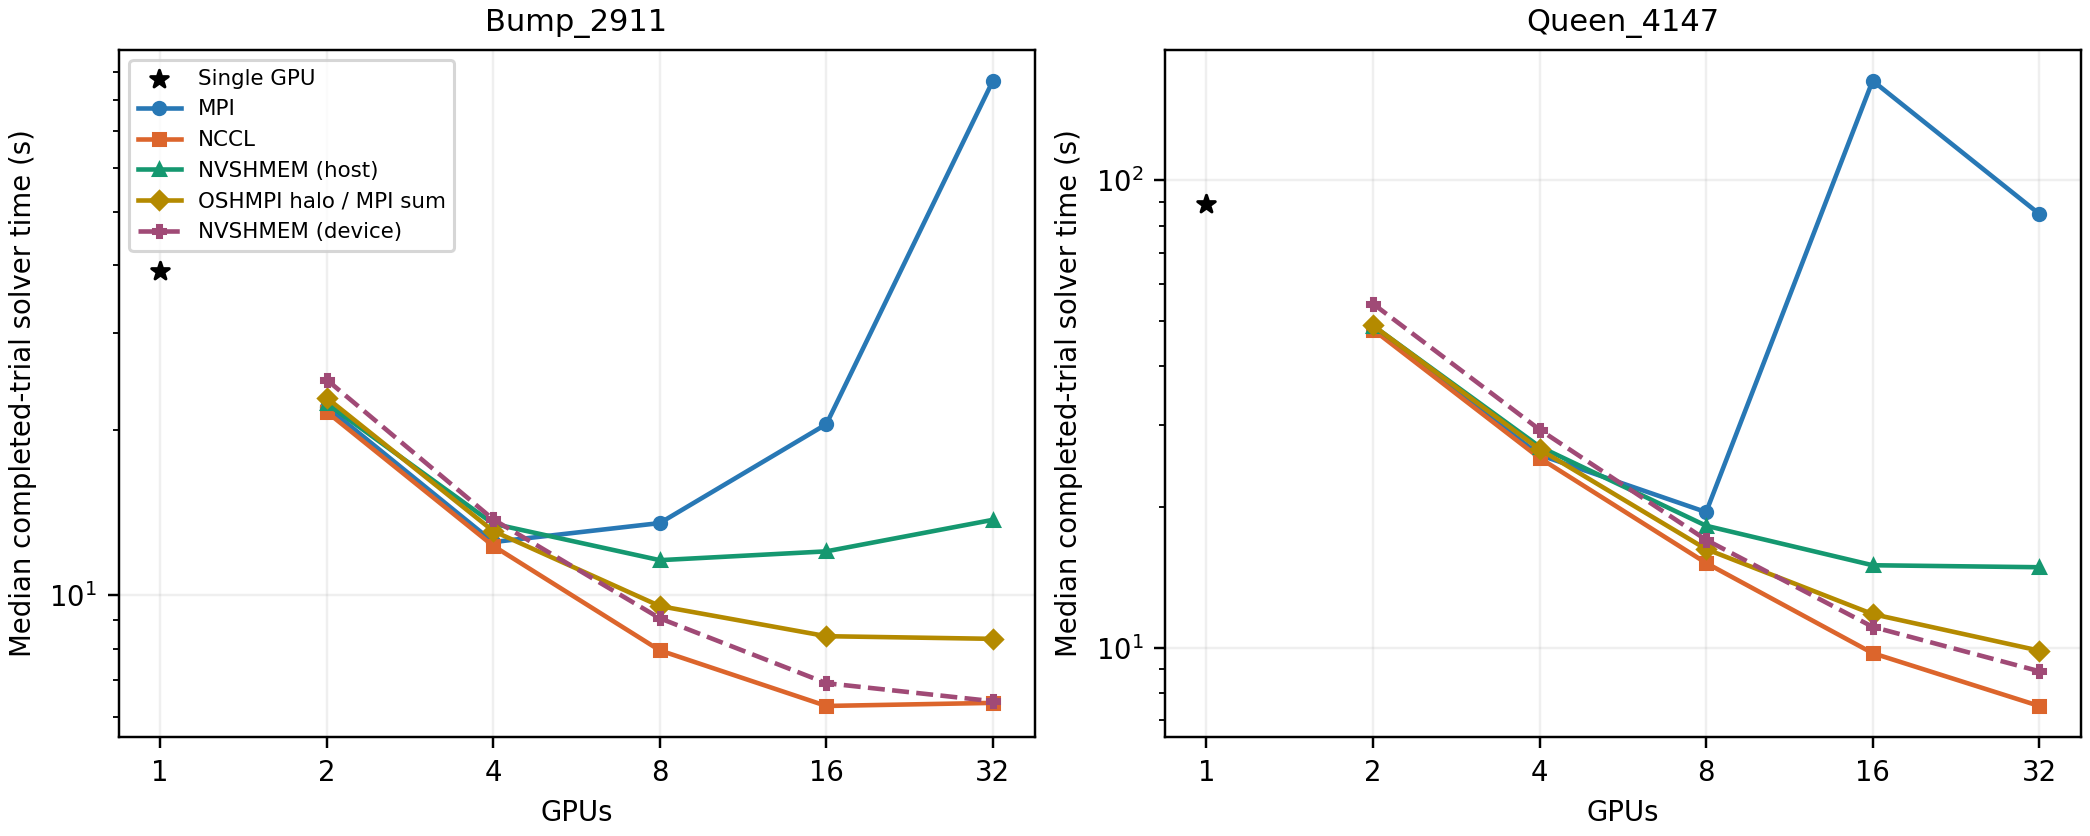
\includegraphics[width=\textwidth]{figures/results/acg-backend-median.png}
\caption[Median aCG solver time of the native paths]{Median solver time over retained residual-valid completed trials for all native aCG paths. The device-NVSHMEM series changes solver organization as well as invocation. MPI's large-scale medians expose the slow mode that a fastest-trial curve would hide.}
\label{fig:m-acg-backend-median}
\end{figure}

\begin{table}[htbp]
\centering
\caption[OSHMPI-halo aCG results]{OSHMPI-halo aCG results from the fastest residual-valid trial. Relative columns compare analytical throughput, not solver-time ratios.}
\label{tab:m-acg-oshmpi}
\footnotesize
% Generated by tools/rebuild_main_evidence.py; include outside tabular.
\begin{tabular}{llrrrr}
\toprule
Matrix & GPUs & Time (s) & GFLOP/s/GPU & vs NCCL & vs host NVSHMEM\\
\midrule
Bump & 2 & 22.177 & 162.10 & $-3.1\%$ & $-0.9\%$\\
Bump & 4 & 12.716 & 139.84 & $-4.6\%$ & $+4.3\%$\\
Bump & 8 & 9.185 & 95.33 & $-17.7\%$ & $+20.6\%$\\
Bump & 16 & 8.198 & 53.31 & $-28.2\%$ & $+40.0\%$\\
Bump & 32 & 8.004 & 27.78 & $-25.9\%$ & $+68.6\%$\\
Queen & 2 & 48.311 & 189.13 & $-1.5\%$ & $-0.5\%$\\
Queen & 4 & 26.165 & 175.37 & $-3.0\%$ & $+2.4\%$\\
Queen & 8 & 15.902 & 141.58 & $-6.9\%$ & $+11.4\%$\\
Queen & 16 & 11.666 & 97.38 & $-18.5\%$ & $+25.9\%$\\
Queen & 32 & 9.603 & 59.28 & $-24.9\%$ & $+52.0\%$\\
\bottomrule
\end{tabular}

\end{table}

Figure~\ref{fig:m-acg-scaling} separates the stable scaling trends from MPI variability. The monolithic NVSHMEM solver improves relative to blocking OSHMPI at larger process counts, although NCCL remains ahead in these work-normalized curves. This is consistent with reducing repeated host synchronization under the proxy-assisted configuration of Section~\ref{sec:ibgda-check}, but also reflects changed solver organization.

\begin{figure}[!hbp]
\centering
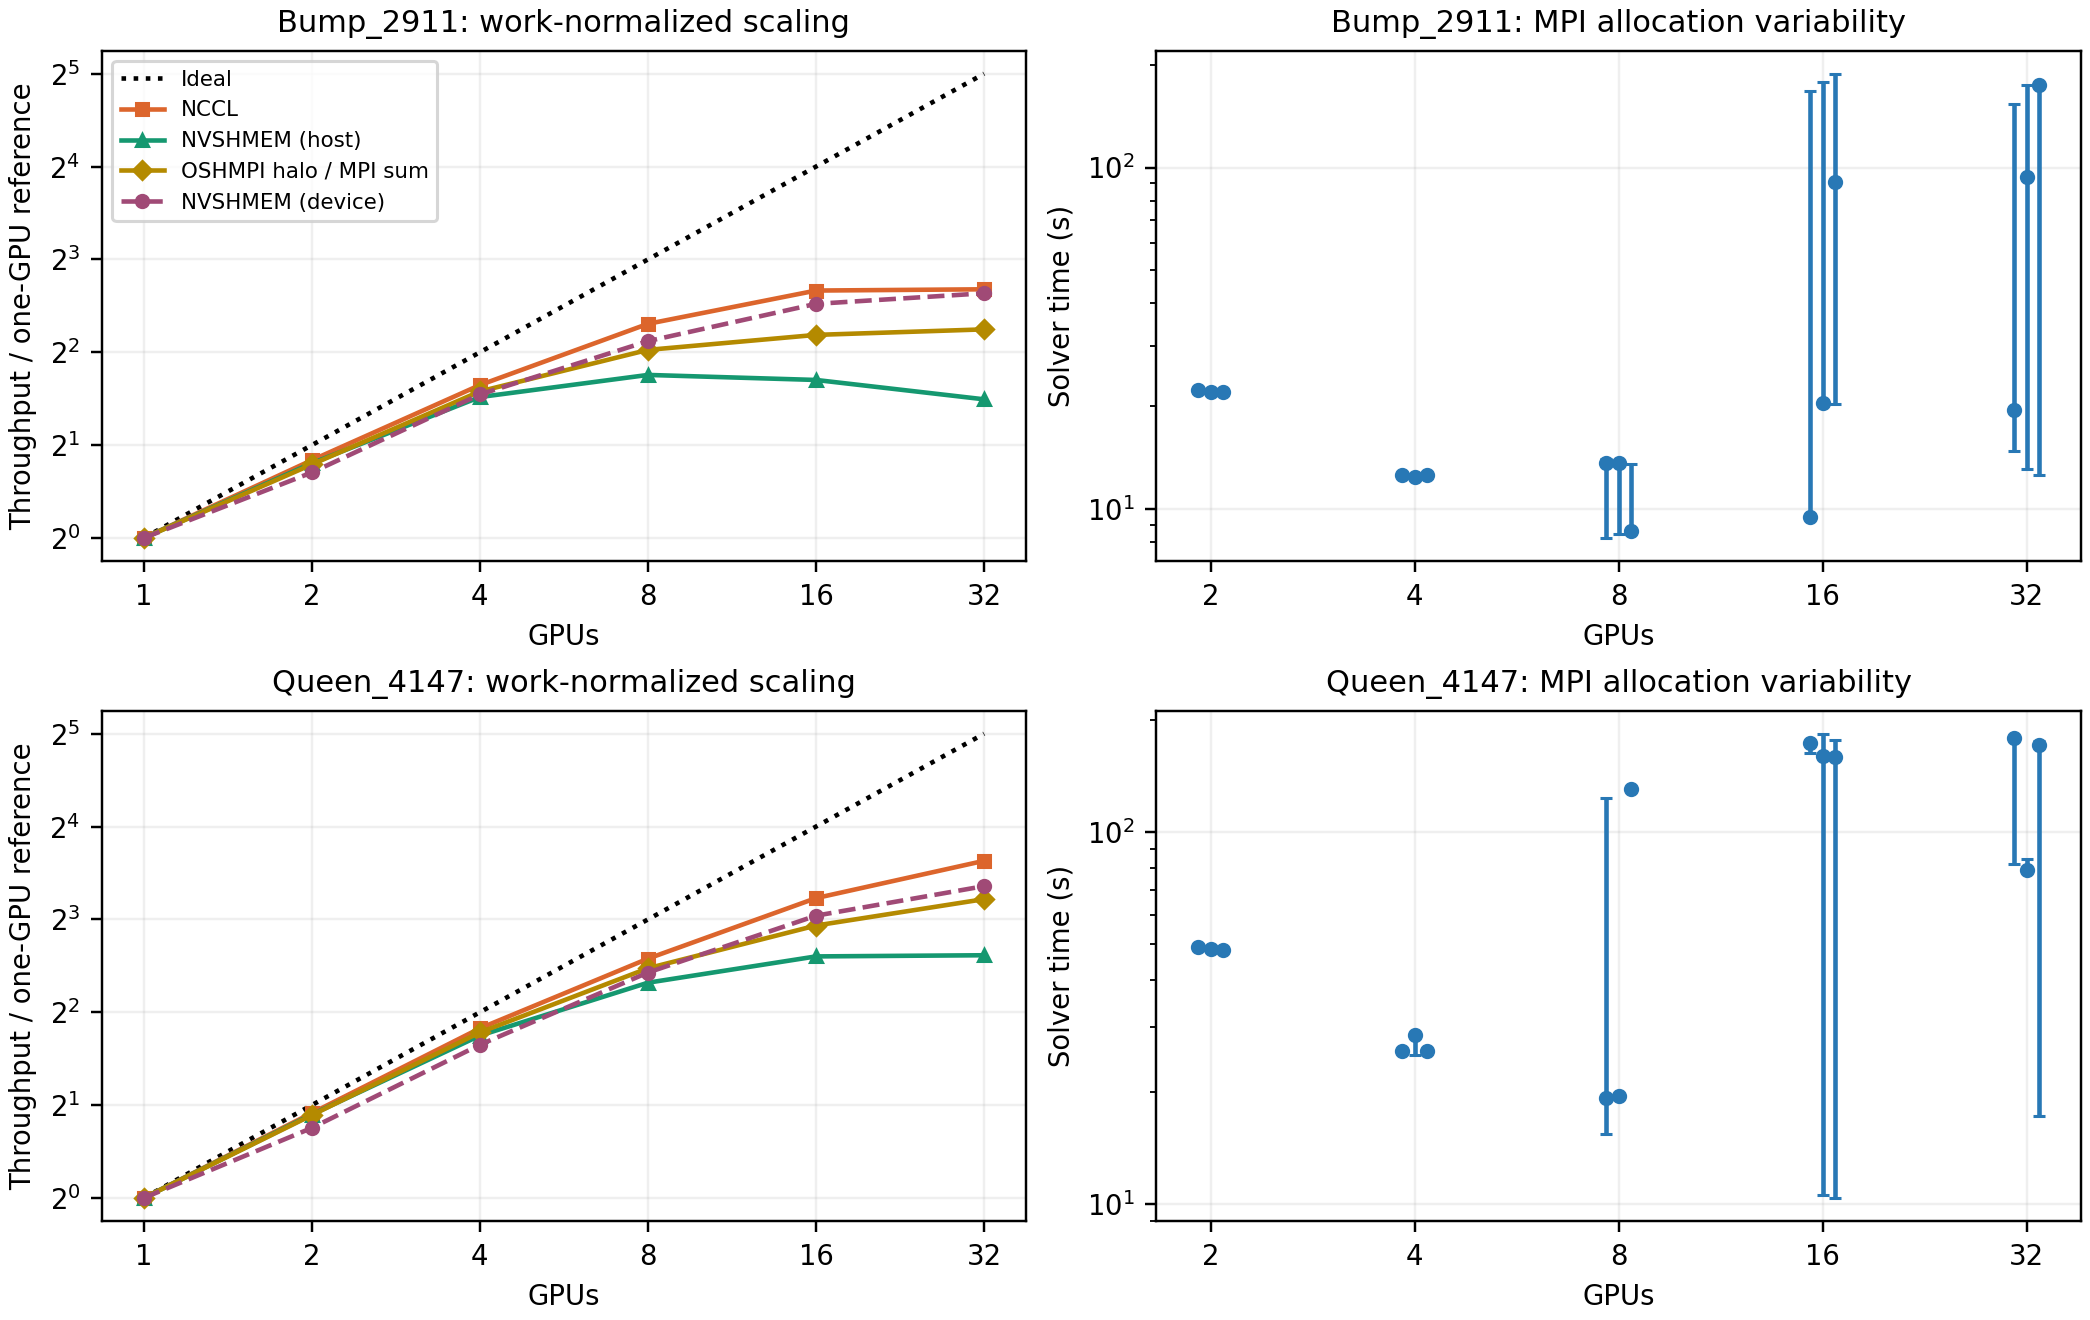
\includegraphics[width=\textwidth]{figures/results/acg-campaign-summary.png}
\caption[aCG scaling and variability]{aCG scaling and variability. Left: analytical throughput of fastest-valid trials normalized to the one-GPU reference. Right: MPI solver time by allocation, with median markers and trial minimum--maximum ranges. The dashed device-NVSHMEM series changes solver organization as well as initiation.}
\label{fig:m-acg-scaling}
\end{figure}

OSHMPI increasingly outperforms the host-NVSHMEM configuration. That result must be read with the application's disabled NCCL dispatch: it compares the installed native NVSHMEM reduction path, not the NCCL-dispatched path used by the default benchmark.

\subsection{Scalar-Reduction Agreement}\label{sec:reduction-agreement}

The most direct comparison between benchmark and solver pairs the operation actually executed rather than the communicator's name (Table~\ref{tab:m-acg-reduction-pairing}). Both the \texttt{cg\_step} benchmark and steady CG iteration perform two separate one-double global sums. The comparison uses half the reduction-phase time in \texttt{cg\_step} and compares it with the application's recorded cost per reduction.

\begin{table}[htbp]
\centering
\caption[Reduction pairings between \texttt{cg\_step} and aCG]{Reduction pairings and remaining configuration differences.}
\label{tab:m-acg-reduction-pairing}
\footnotesize
\begin{tabularx}{\textwidth}{lYY}
\toprule
\texttt{cg\_step} path & Application path & Interpretation\\
\midrule
CUDA MPI & MPI scalar calls with OSHMPI halo & Avoids mixing the unstable MPI halo into the reference\\
CUDA NCCL & NCCL communicator & Same scalar collective interface\\
CUDA NVSHMEM & Host-NVSHMEM communicator & NCCL dispatch differs in the default archive\\
Direct OSHMPI & No matched archived scalar path & Benchmark stages to host; application reduces through MPI\\
\bottomrule
\end{tabularx}
\end{table}

The mean discrepancies range from 7.8\% to 11.1\% (Table~\ref{tab:m-acg-reduction-correlation}). Individual cells can differ more: the NCCL Bump estimate is approximately 20\% high at eight and 16 GPUs. Figure~\ref{fig:m-acg-reduction-prediction} shows this variation. The comparison supports approximate agreement for these scalar reductions, while the application timing also includes differences in when ranks reach the operation. No model is fitted or tested on held-out cases, so these percentages do not quantify prediction accuracy for other workloads or for total solver time.

\begin{table}[!hbp]
\centering
\caption[Scalar-reduction discrepancy between \texttt{cg\_step} and aCG]{Mean absolute percentage discrepancy over five measured rank counts, regenerated from the retained benchmark--solver pairs.}
\label{tab:m-acg-reduction-correlation}
% Generated by tools/rebuild_main_evidence.py; include outside tabular.
\begin{tabular}{lrr}
\toprule
Reduction path & Bump\_2911 & Queen\_4147\\
\midrule
MPI & 9.2\% & 11.1\%\\
NCCL & 10.5\% & 7.8\%\\
\bottomrule
\end{tabular}

\end{table}

\begin{figure}[!hbp]
\centering
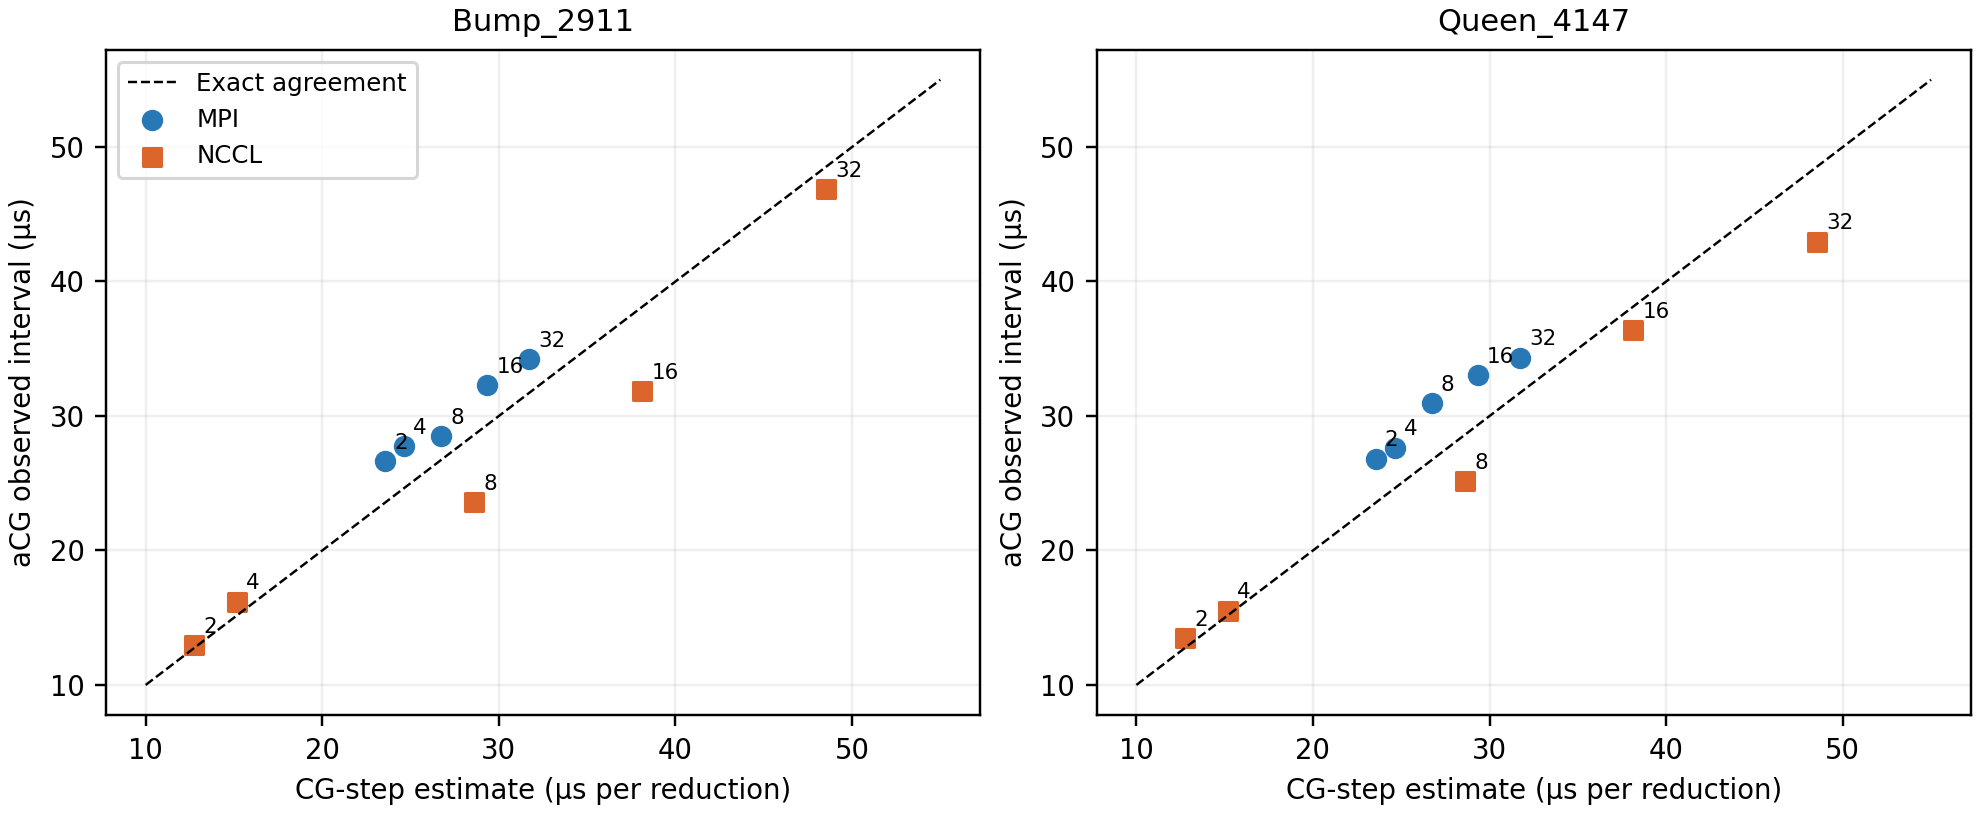
\includegraphics[width=\textwidth]{figures/results/acg-reduction-prediction.png}
\caption[\texttt{cg\_step} estimate versus aCG measurement]{One-double reduction estimate from \texttt{cg\_step} versus aCG measurement. Point labels give GPU count. The dashed line is exact agreement; no model is fitted to these points. MPI observations come from the OSHMPI-halo solver.}
\label{fig:m-acg-reduction-prediction}
\end{figure}

The auxiliary configuration analysis reports that disabling NCCL dispatch materially changes NVSHMEM reduction time and gives matched errors of approximately 14--21\%. The matched per-trial arm is not present in the imported default \ac{JSON} record, so it is not plotted as an independently regenerated prediction. Repeating that control with explicit metadata would bring NVSHMEM to the same reproducibility level as the MPI/NCCL pairs. The separately recorded UCX-threshold control changes the MPI \texttt{cg\_step} time by only approximately 2--3\%, which is too small to explain the much larger application variability.


\subsection{Device-Initiated Scaling Agreement}\label{sec:cg-device-correlation}

The device-initiated implementation supports a second comparison between benchmark and solver, on a different quantity. Neither the device benchmark nor the monolithic device solver records phase timers, so the reduction comparison of Section~\ref{sec:reduction-agreement} cannot be repeated for them. What both expose is whole-iteration time: the benchmark's step time and the solver's time per iteration. They solve different problems, so only their strong-scaling shape is comparable, and each series is normalized to its own two-GPU value before being compared.

Figure~\ref{fig:m-cg-device-scaling} shows how the agreement changes with benchmark size. At side 8192, the benchmark time falls to 0.20 of its two-GPU value at 32 GPUs. The solver reaches 0.26 on Bump\_2911 and 0.16 on Queen\_4147. The mean absolute deviations are 8.0\% and 12.6\%, respectively (Table~\ref{tab:m-cg-device-correlation}). At side 512, the benchmark instead grows to 3.55 times its two-GPU time, with deviations of 582\% and 853\%. This smaller problem leaves less local work per GPU, making communication and synchronization more prominent as GPUs are added.

\begin{figure}[!hbp]
\centering
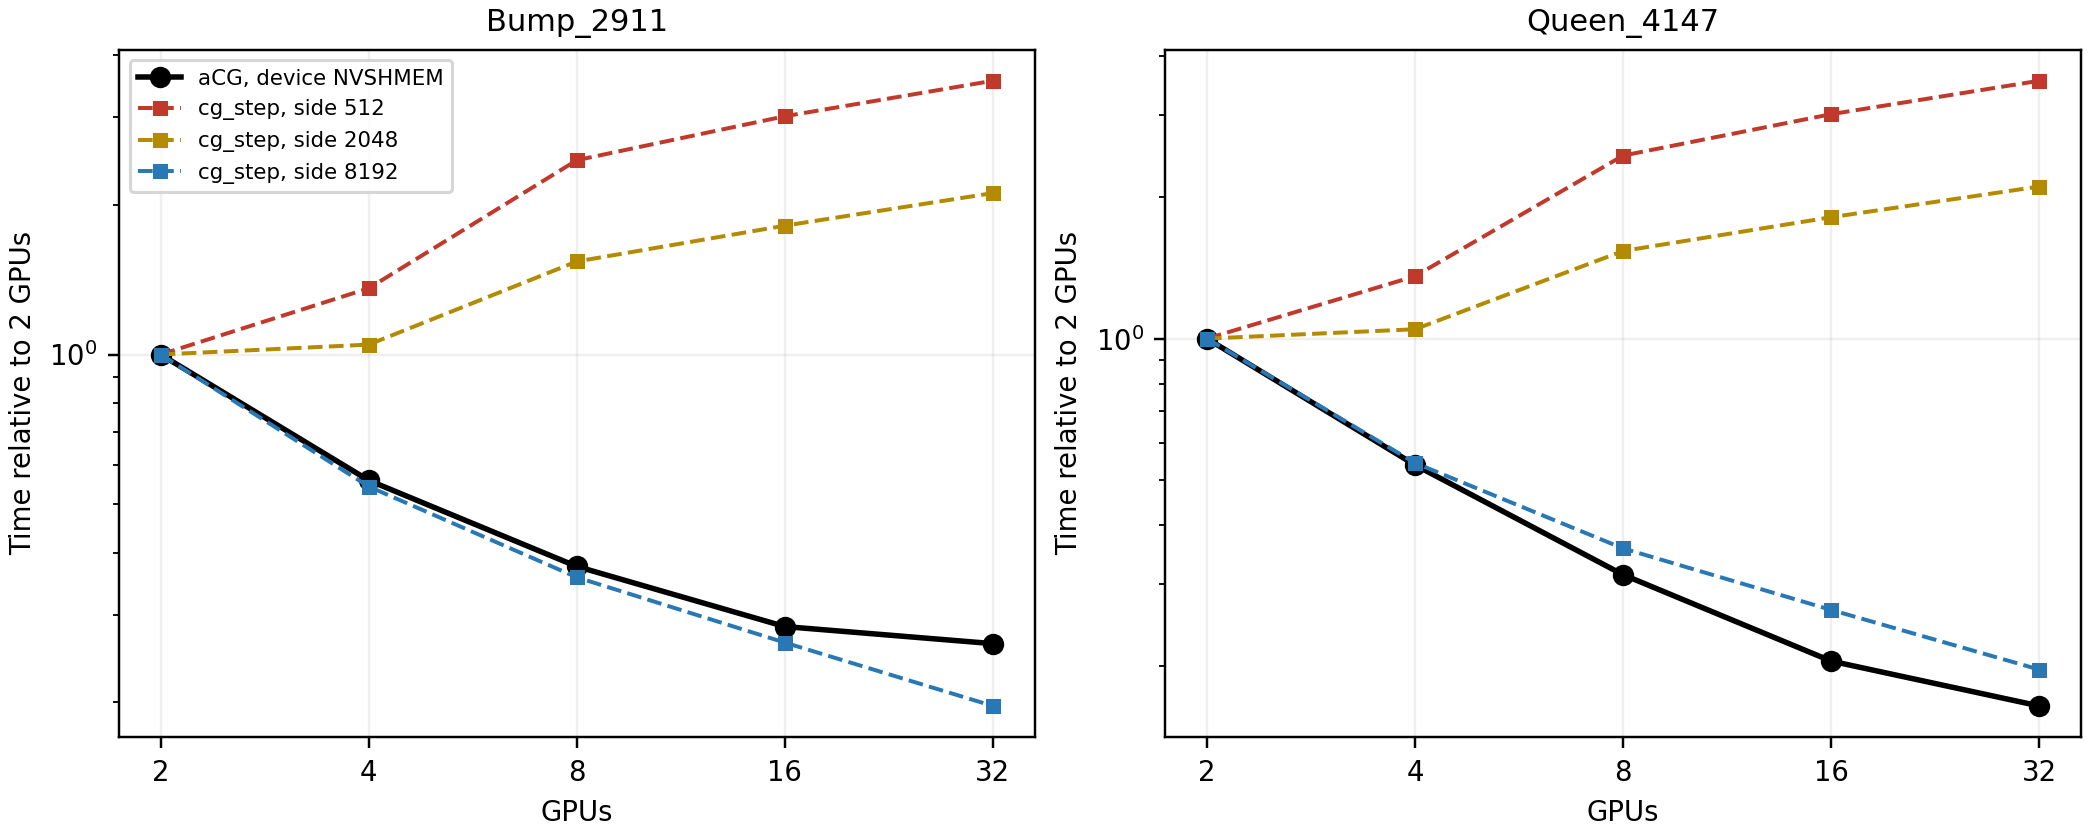
\includegraphics[width=\textwidth]{figures/results/cg-device-scaling.png}
\caption[Strong scaling of the device-initiated \texttt{cg\_step} and the device-NVSHMEM solver]{Strong scaling of the device-initiated \texttt{cg\_step} at three grid sides against the device-NVSHMEM solver, each normalized to its own two-GPU value. Lower is better; a series that rises does not scale.}
\label{fig:m-cg-device-scaling}
\end{figure}

\begin{table}[!hbp]
\centering
\caption[Strong-scaling deviation of the device-initiated \texttt{cg\_step}]{Mean absolute deviation between the normalized strong-scaling curves of the device-initiated \texttt{cg\_step} and the device-NVSHMEM solver, by grid side.}
\label{tab:m-cg-device-correlation}
\footnotesize
% Generated by tools/import_cg_device_evidence.py; include outside tabular.
\begin{tabular}{rrr}
\toprule
Grid side & Bump\_2911 & Queen\_4147\\
\midrule
512 & 582.2\% & 852.6\%\\
1024 & 490.2\% & 723.0\%\\
2048 & 328.2\% & 490.7\%\\
4096 & 56.0\% & 104.8\%\\
8192 & 8.0\% & 12.6\%\\
\bottomrule
\end{tabular}

\end{table}

The practical lesson is to match local computation as well as communication. The side-8192 benchmark resembles the solver's scaling, while the side-512 benchmark predicts the opposite trend. Using a small problem to emphasize communication costs can therefore make a benchmark less representative of an application with more work per GPU. This extends the comparison in Section~\ref{sec:cg-comparison-micro} to GPU-initiated execution.


\subsection{Halo Structure and Overlap}

The regular halo test and the \texttt{cg\_step} benchmark do not reproduce aCG's exchange. The \texttt{cg\_step} benchmark has at most two fixed neighbors and a small structured payload. Table~\ref{tab:m-acg-halo-signatures} reconstructs the application signatures from the stored communication matrices, with element-to-byte conversion checked against the per-rank log totals. Bump reaches a mean of 10.8 outgoing neighbors at 32 GPUs, with as many as 17 on an individual rank. These asymmetric graphs are available as replay inputs in the reconciled archive. Nonblocking MPI and NCCL paths may progress while local SpMV executes, whereas the measured OSHMPI path completes before that work begins.

\begin{table}[htbp]
\centering
\caption[aCG halo signatures from the sparse partitions]{Application halo signatures reconstructed from the fixed sparse partitions. Volume is mean outgoing KiB per rank and exchange, excluding reductions.}
\label{tab:m-acg-halo-signatures}
\footnotesize
% Generated by tools/rebuild_main_evidence.py; include outside tabular.
\begin{tabular}{lrrrr}
\toprule
Matrix & GPUs & Mean neighbors & Max neighbors & Send KiB/rank\\
\midrule
Bump & 4 & 3.0 & 3 & 282.7\\
Bump & 16 & 9.0 & 12 & 175.1\\
Bump & 32 & 10.8 & 17 & 122.0\\
Queen & 4 & 3.0 & 3 & 328.3\\
Queen & 16 & 6.4 & 10 & 226.4\\
Queen & 32 & 7.8 & 14 & 156.9\\
\bottomrule
\end{tabular}

\end{table}

The nominal halo timer cannot resolve this difference by itself. It measures only the wait at halo-end. For OSHMPI, communication has already completed in halo-begin, so a small halo column coexists with a substantial cost in \emph{other}. Dividing the full payload by that residual wait produces an apparent bandwidth, not a physical transfer rate. A comparison of isolated halo latency with this column would therefore compare different intervals.

Auxiliary attempts to replace global barriers with neighbor flags or to split begin/end without deferring completion did not improve total solver time. They show why a change in timer placement is insufficient to create overlap. A useful next comparison must retain the same peer graph and measure submission, progress, completion, and exposed wait around independent local work.

These differences explain why the fastest backend in the \texttt{cg\_step} benchmark need not give the fastest solver. The reduction operation and result location change, as do the halo peers and opportunities for overlap. The measurements do not separate how much each factor contributes to the ranking reversal.

\subsection{Convergence and Variability}\label{sec:acg-variability}

All 507 retained completed logs meet the recorded relative residual criterion, including 90 OSHMPI trials. This validates the recorded numerical outcome of those runs; it does not imply that every attempted run completed or that floating-point reduction order leaves iteration counts unchanged. Both total time and executed work are retained so that convergence differences remain visible.

MPI shows a separate performance-variability problem: some native-solver runs take much longer than others, a behavior referred to here as the \emph{slow mode}. It describes an observed timing pattern, not a runtime setting. The halo and subsequent allreduce intervals grow together in these runs. In contrast, the OSHMPI-halo solver uses the same MPI scalar interface with much more stable reduction timings. This points to the surrounding exchange and differences in when ranks reach the reduction, without isolating a particular UCX state or progress mechanism.

Large variations also occur among trials within one allocation, as Figure~\ref{fig:m-acg-scaling} shows. Node selection alone is therefore insufficient to explain the effect. Valid solutions can coexist with timing decompositions whose overlapping event regions are unsuitable for phase attribution. The chapter consequently reports MPI allocation ranges and avoids presenting its rare fastest run as a representative scaling curve. The irregular-halo replay is intended to test whether the behavior can be reproduced outside the complete solver.

\subsection{Native and Portable Solver Comparison}\label{sec:acg-sycl}

This comparison addresses the portability part of RQ3: how much native CUDA performance does the SYCL solver retain on the same hardware? Both implementations were run in the same allocations to reduce differences caused by node selection and network conditions. The earlier native campaign provides a separate reference. The two comparisons answer different questions and are discussed separately below.

The paired runs share nodes, partitions, the MPI installation, and Open MPI and UCX settings (Section~\ref{sec:acg-environment}). Toolchains differ, and the oneCCL/NCCL comparison also changes the NCCL release and halo implementation. One \texttt{2n4g} allocation on Bump\_2911 failed for every run of both solvers with the same UCX error. Excluding it leaves two allocations for that case and three for every other case. All 192 completed trials on each side meet the residual criterion; the SYCL residual is independently recomputed on the host.

Table~\ref{tab:m-acg-sycl} reports the SYCL-to-native solver-time ratio calculated within allocations, following Section~\ref{sec:acg-environment}. Ratios below one favor SYCL. Time-per-iteration ratios agree with solver-time ratios within 2\%, except on Queen\_4147 with one GPU, where SYCL takes 2.3\% more iterations.

\begin{figure}[htbp]
\centering
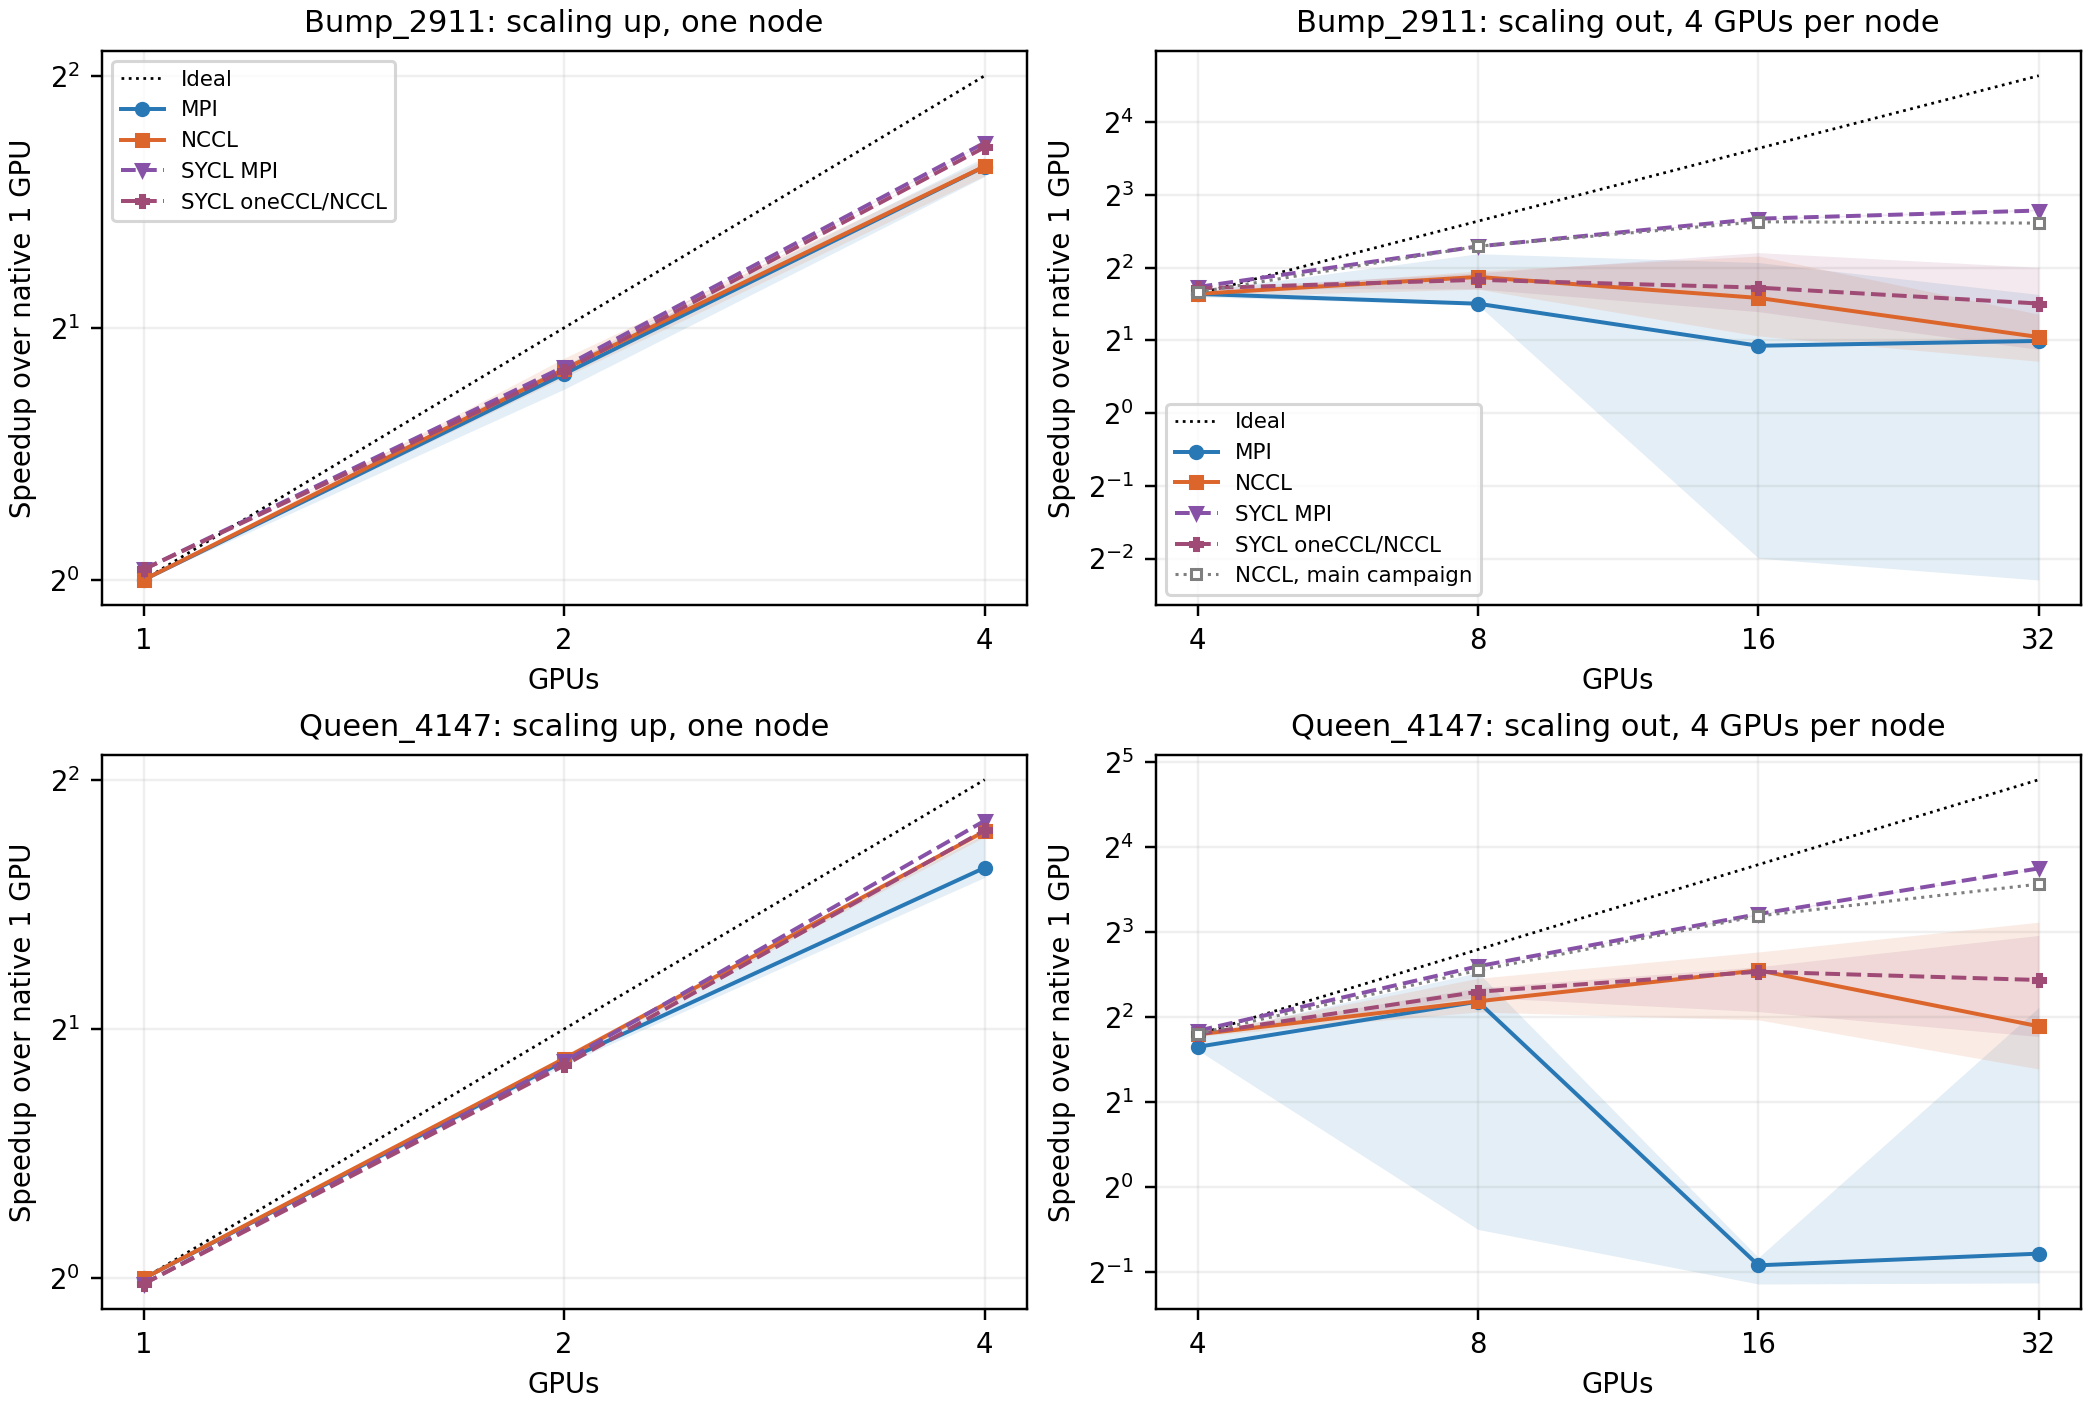
\includegraphics[width=\textwidth]{figures/results/acg-sycl-scaling.png}
\caption[Strong scaling of the native and SYCL aCG solvers]{Strong scaling of the native and SYCL solvers from the same allocations, as speedup over the native single-GPU median solver time. Left: scaling up within one node. Right: scaling out with four GPUs per node. Lines are medians, shading spans the trial minimum and maximum; the dotted gray series is native NCCL from the main campaign, shown for reference. SYCL oneCCL/NCCL reduces through NCCL but exchanges its halo through MPI.}
\label{fig:m-acg-sycl-scaling}
\end{figure}

\begin{table}[htbp]
\centering
\caption[Native and SYCL aCG solver times]{Median solver time in seconds of each native aCG variant and its SYCL counterpart, from the same allocations, and the median over allocations of their per-allocation ratio, SYCL over CUDA; ratios above one favor CUDA. At one GPU the single-GPU solvers are compared, in the MPI columns.}
\label{tab:m-acg-sycl}
\footnotesize
% Generated by tools/import_acg_sycl_evidence.py; include outside tabular.
\begin{tabular}{lrrrrrrr}
\toprule
Matrix & GPUs & MPI & SYCL MPI & Ratio & NCCL & oneCCL/NCCL & Ratio\\
\midrule
Bump\_2911 & 1 & 39.0 & 37.9 & $0.97$ & -- & -- & --\\
 & 2 & 22.1 & 21.7 & $0.98$ & 21.8 & 21.9 & $1.00$\\
 & 4 & 12.5 & 11.7 & $0.94$ & 12.5 & 11.9 & $0.95$\\
 & 8 & 13.7 & 8.0 & $0.75$ & 10.6 & 10.9 & $1.03$\\
 & 16 & 20.5 & 6.1 & $0.30$ & 13.0 & 11.8 & $0.74$\\
 & 32 & 19.6 & 5.6 & $0.29$ & 18.9 & 13.7 & $0.77$\\
\midrule
Queen\_4147 & 1 & 88.8 & 90.2 & $1.02$ & -- & -- & --\\
 & 2 & 48.5 & 48.6 & $1.00$ & 48.2 & 49.1 & $1.02$\\
 & 4 & 28.4 & 24.9 & $0.87$ & 25.6 & 25.6 & $0.99$\\
 & 8 & 19.6 & 14.7 & $0.75$ & 19.6 & 18.1 & $0.92$\\
 & 16 & 168.8 & 9.6 & $0.06$ & 15.2 & 15.4 & $0.98$\\
 & 32 & 153.5 & 6.6 & $0.04$ & 24.0 & 16.4 & $0.83$\\
\bottomrule
\end{tabular}

\end{table}

\begin{figure}[htbp]
\centering
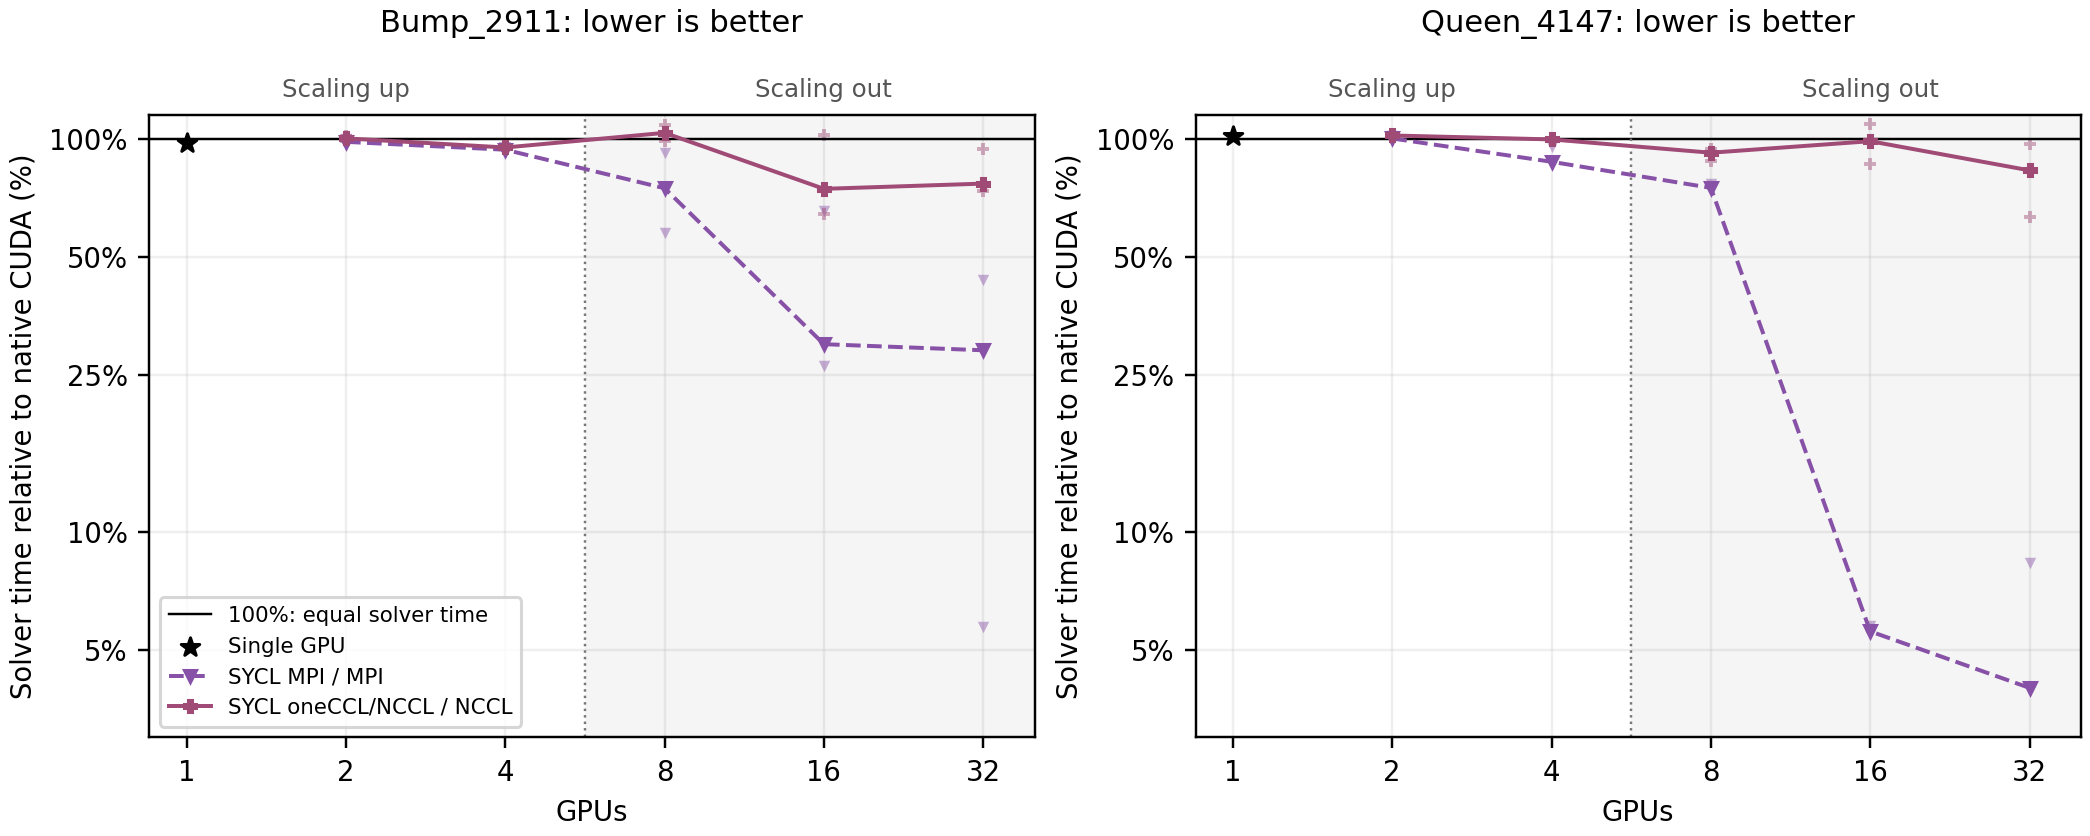
\includegraphics[width=\textwidth]{figures/results/acg-sycl-ratio.png}
\caption[Change in SYCL solver time relative to native CUDA]{Percentage change in SYCL solver time relative to native CUDA at the same GPU count, $100\,(T_{\mathrm{SYCL}}/T_{\mathrm{CUDA}}-1)$. Points are single allocations, each comparing the SYCL and native medians of that job; lines are medians over allocations. Values below the 0\% line mean SYCL takes less time; a change of $-50\%$ corresponds to a twofold speedup, so the axis is not a percentage speedup. The shaded region marks scaling out. The large MPI reductions there reflect unusually slow native MPI runs; this is a runtime comparison, not parallel efficiency.}
\label{fig:m-acg-sycl-ratio}
\end{figure}

Scaling up, SYCL solver times range from 0.87 to 1.02 times the native CUDA times across both matrices and reduction implementations (Figure~\ref{fig:m-acg-sycl-scaling}, left). The only ratio below 0.93 is Queen\_4147 with MPI on four GPUs. Native MPI varies between those allocations, while the SYCL trials agree within 0.1\%. The native NCCL medians are also close to the main campaign: 12.5 versus 12.3\,s on Bump\_2911 and 25.6 versus 25.5\,s on Queen\_4147 at four GPUs.

Scaling out with MPI, the SYCL solver continues strong scaling on both matrices (Figure~\ref{fig:m-acg-sycl-scaling}, right). At \texttt{2n4g}, \texttt{4n4g}, and \texttt{8n4g}, its times fall from 8.0 to 6.1 to 5.6\,s on Bump\_2911. On Queen\_4147 they fall from 14.7 to 9.6 to 6.6\,s. Native MPI instead shows the slow runs described in Section~\ref{sec:acg-variability}, with Queen\_4147 medians of 169 and 153\,s at \texttt{4n4g} and \texttt{8n4g}. These slow runs account for the unusually low SYCL-to-native ratios of 0.04--0.75. No SYCL MPI trial shows the same behavior despite sharing the nodes and MPI settings. This points to an interaction with how the native solver drives communication, without isolating its cause.

Scaling out with NCCL, the paired results give SYCL-to-native ratios of 0.74--1.03, a change in solver time of $-26\%$ to $+3\%$ (Figure~\ref{fig:m-acg-sycl-ratio}). In these allocations, the SYCL oneCCL/NCCL solver is generally as fast as or faster than the native NCCL solver. This comparison includes differences in NCCL version, halo exchange, and synchronization as well as the programming interface.

Comparing against the earlier native campaign gives a different picture. At \texttt{8n4g}, native NCCL takes 18.9\,s on Bump\_2911 in the paired campaign, compared with 6.4\,s before; Queen\_4147 takes 24.0 versus 7.5\,s. Relative to those earlier native medians, SYCL oneCCL/NCCL takes 1.19--2.19 times as long across \texttt{2n4g}--\texttt{8n4g}. The baseline changes substantially between campaigns, so that ratio is not an isolated measure of SYCL overhead.

NCCL selected InfiniBand with GPUDirect RDMA in the paired jobs. A later check at \texttt{2n4g}, outside the archive, gave 9.1\,s for native NCCL and 9.4\,s for SYCL oneCCL/NCCL. Both improved together, consistent with allocation-dependent variation. SYCL MPI's \texttt{8n4g} medians of 5.6 and 6.6\,s are also lower than the fastest main-campaign NCCL trials, at 6.0 and 7.25\,s. These separate-campaign observations provide context, but a matched comparison would be needed to rank the implementations on that basis.

The phase timings identify a more specific difference within the SYCL solver. Its MPI and oneCCL/NCCL variants use identical computational kernels and MPI halo exchanges. Across nodes, the oneCCL/NCCL variant spends 85--340\,$\mu$s more per iteration blocked in the two scalar reductions; within one node, the difference is 8--22\,$\mu$s. The host waits for the oneCCL event and queue after each reduction. Native NCCL instead orders the reductions with subsequent work on the GPU stream, without a host wait for each one. These measurements identify additional waiting in the adapter, while allocation differences also affect the cross-campaign solver-time ratios.

Several shared design choices help explain why the within-node timings are close. Both solvers use the same partition and split each rank's matrix into an interior block and a halo block. The interior product uses cuSPARSE with 32-bit indices. Each solver packs its outgoing halo values in one kernel and overlaps the exchange with the interior SpMV. Both keep CG scalars in device memory and form $\alpha$ and $\beta$ inside the vector-update kernels. One small result is copied to the host per iteration for convergence testing, while the search-direction update can proceed.

The implementations still differ in how they coordinate this work. The SYCL solver uses DPC++ and oneMath on one in-order queue, with host waits before MPI accesses produced data, at communication completion, and for convergence readback. Native aCG uses a separate CUDA stream and events for halo exchange. Its NCCL variant also exchanges halos through NCCL, while both SYCL variants use MPI. The paired results show that these design differences coexist with close within-node performance; the phase timings highlight reduction waits as an important multi-node cost.

\begin{keypoint}[CUDA--SYCL takeaway]
Scaling up, the SYCL solver takes 0.87--1.02 times the native CUDA solver time. Scaling out, SYCL MPI continues strong scaling to 32 GPUs, while native MPI exhibits slow runs. SYCL oneCCL/NCCL takes 0.74--1.03 times the native NCCL time in the same allocations, but 1.19--2.19 times the main campaign's native NCCL time. Its reductions introduce additional host waits, while the cross-campaign comparison also includes allocation differences.
\end{keypoint}
